\documentclass[10pt,journal,compsoc]{IEEEtran}

\usepackage[utf8]{inputenc}


\usepackage{booktabs}
\usepackage[usenames]{color}
\usepackage{blindtext}
\definecolor{darkgray}{RGB}{90,90,90}
\definecolor{lightgray}{RGB}{210,210,210}
\newcommand\xbar[1]{#1 {\color{darkgray} \rule{\dimexpr #1pt * 16}{5.5pt}}{\color{lightgray} \rule{\dimexpr 16pt - (#1pt * 16)}{5.5pt}}}

\definecolor{codegray}{gray}{0.9}
\newcommand{\code}[1]{\colorbox{codegray}{\texttt{#1}}}
\newcommand{\codeinl}[1]{%
  \begingroup
  \setlength{\fboxsep}{2pt}%
  \mbox{\vphantom{#1}\smash{\colorbox{codegray}{\texttt{#1}}}}%
  \endgroup
}

\newcommand{\todo}[1]{\textcolor{red}{TODO: #1}}

% Some very useful LaTeX packages include:
% (uncomment the ones you want to load)


% *** MISC UTILITY PACKAGES ***
%
%\usepackage{ifpdf}
% Heiko Oberdiek's ifpdf.sty is very useful if you need conditional
% compilation based on whether the output is pdf or dvi.
% usage:
% \ifpdf
%   % pdf code
% \else
%   % dvi code
% \fi
% The latest version of ifpdf.sty can be obtained from:
% http://www.ctan.org/pkg/ifpdf
% Also, note that IEEEtran.cls V1.7 and later provides a builtin
% \ifCLASSINFOpdf conditional that works the same way.
% When switching from latex to pdflatex and vice-versa, the compiler may
% have to be run twice to clear warning/error messages.






% *** CITATION PACKAGES ***
%
\ifCLASSOPTIONcompsoc
  % IEEE Computer Society needs nocompress option
  % requires cite.sty v4.0 or later (November 2003)
  \usepackage[nocompress]{cite}
\else
  % normal IEEE
  \usepackage{cite}
\fi
% cite.sty was written by Donald Arseneau
% V1.6 and later of IEEEtran pre-defines the format of the cite.sty package
% \cite{} output to follow that of the IEEE. Loading the cite package will
% result in citation numbers being automatically sorted and properly
% "compressed/ranged". e.g., [1], [9], [2], [7], [5], [6] without using
% cite.sty will become [1], [2], [5]--[7], [9] using cite.sty. cite.sty's
% \cite will automatically add leading space, if needed. Use cite.sty's
% noadjust option (cite.sty V3.8 and later) if you want to turn this off
% such as if a citation ever needs to be enclosed in parenthesis.
% cite.sty is already installed on most LaTeX systems. Be sure and use
% version 5.0 (2009-03-20) and later if using hyperref.sty.
% The latest version can be obtained at:
% http://www.ctan.org/pkg/cite
% The documentation is contained in the cite.sty file itself.
%
% Note that some packages require special options to format as the Computer
% Society requires. In particular, Computer Society  papers do not use
% compressed citation ranges as is done in typical IEEE papers
% (e.g., [1]-[4]). Instead, they list every citation separately in order
% (e.g., [1], [2], [3], [4]). To get the latter we need to load the cite
% package with the nocompress option which is supported by cite.sty v4.0
% and later. Note also the use of a CLASSOPTION conditional provided by
% IEEEtran.cls V1.7 and later.





% *** GRAPHICS RELATED PACKAGES ***
%
\ifCLASSINFOpdf
  \usepackage[pdftex]{graphicx}
  % declare the path(s) where your graphic files are
  % \graphicspath{{../pdf/}{../jpeg/}}
  % and their extensions so you won't have to specify these with
  % every instance of \includegraphics
  % \DeclareGraphicsExtensions{.pdf,.jpeg,.png}
\else
  % or other class option (dvipsone, dvipdf, if not using dvips). graphicx
  % will default to the driver specified in the system graphics.cfg if no
  % driver is specified.
  \usepackage[dvips]{graphicx}
  % declare the path(s) where your graphic files are
  % \graphicspath{{../eps/}}
  % and their extensions so you won't have to specify these with
  % every instance of \includegraphics
  % \DeclareGraphicsExtensions{.eps}
\fi
% graphicx was written by David Carlisle and Sebastian Rahtz. It is
% required if you want graphics, photos, etc. graphicx.sty is already
% installed on most LaTeX systems. The latest version and documentation
% can be obtained at: 
% http://www.ctan.org/pkg/graphicx
% Another good source of documentation is "Using Imported Graphics in
% LaTeX2e" by Keith Reckdahl which can be found at:
% http://www.ctan.org/pkg/epslatex
%
% latex, and pdflatex in dvi mode, support graphics in encapsulated
% postscript (.eps) format. pdflatex in pdf mode supports graphics
% in .pdf, .jpeg, .png and .mps (metapost) formats. Users should ensure
% that all non-photo figures use a vector format (.eps, .pdf, .mps) and
% not a bitmapped formats (.jpeg, .png). The IEEE frowns on bitmapped formats
% which can result in "jaggedy"/blurry rendering of lines and letters as
% well as large increases in file sizes.
%
% You can find documentation about the pdfTeX application at:
% http://www.tug.org/applications/pdftex






% *** MATH PACKAGES ***
%
\usepackage{amsmath}
% A popular package from the American Mathematical Society that provides
% many useful and powerful commands for dealing with mathematics.
%
% Note that the amsmath package sets \interdisplaylinepenalty to 10000
% thus preventing page breaks from occurring within multiline equations. Use:
%\interdisplaylinepenalty=2500
% after loading amsmath to restore such page breaks as IEEEtran.cls normally
% does. amsmath.sty is already installed on most LaTeX systems. The latest
% version and documentation can be obtained at:
% http://www.ctan.org/pkg/amsmath

\usepackage{amssymb}

\DeclareMathOperator{\rdname}{name}
\DeclareMathOperator{\rdparent}{\pi}
\DeclareMathOperator{\rdsig}{ident}
\DeclareMathOperator{\rdsub}{subtype}
\DeclareMathOperator{\rdtype}{type}
\DeclareMathOperator{\rdsim}{sim}
\DeclareMathOperator{\rdsimx}{sim_{p}}
\DeclareMathOperator{\rduses}{uses}



\usepackage{listings}
\usepackage{lipsum}
\usepackage{courier}
\definecolor{javablue}{rgb}{0.25,0,1} % for strings
\definecolor{javagreen}{rgb}{0.25,0.5,0.35} % comments
\definecolor{javapurple}{rgb}{0.5,0,0.35} % keywords
\definecolor{javadocblue}{rgb}{0.25,0.35,0.75} % javadoc
\lstset{
language=Java,
basicstyle=\footnotesize\ttfamily,
breaklines=true,
keywordstyle=\color{javapurple}\bfseries,
stringstyle=\color{javablue},
commentstyle=\color{javagreen},
morecomment=[s][\color{javadocblue}]{/**}{*/},
tabsize=2,
frame=single}



% *** SPECIALIZED LIST PACKAGES ***
%
%\usepackage{algorithmic}
% algorithmic.sty was written by Peter Williams and Rogerio Brito.
% This package provides an algorithmic environment fo describing algorithms.
% You can use the algorithmic environment in-text or within a figure
% environment to provide for a floating algorithm. Do NOT use the algorithm
% floating environment provided by algorithm.sty (by the same authors) or
% algorithm2e.sty (by Christophe Fiorio) as the IEEE does not use dedicated
% algorithm float types and packages that provide these will not provide
% correct IEEE style captions. The latest version and documentation of
% algorithmic.sty can be obtained at:
% http://www.ctan.org/pkg/algorithms
% Also of interest may be the (relatively newer and more customizable)
% algorithmicx.sty package by Szasz Janos:
% http://www.ctan.org/pkg/algorithmicx




% *** ALIGNMENT PACKAGES ***
%
\usepackage{array}
% Frank Mittelbach's and David Carlisle's array.sty patches and improves
% the standard LaTeX2e array and tabular environments to provide better
% appearance and additional user controls. As the default LaTeX2e table
% generation code is lacking to the point of almost being broken with
% respect to the quality of the end results, all users are strongly
% advised to use an enhanced (at the very least that provided by array.sty)
% set of table tools. array.sty is already installed on most systems. The
% latest version and documentation can be obtained at:
% http://www.ctan.org/pkg/array


% IEEEtran contains the IEEEeqnarray family of commands that can be used to
% generate multiline equations as well as matrices, tables, etc., of high
% quality.




% *** SUBFIGURE PACKAGES ***
%\ifCLASSOPTIONcompsoc
%  \usepackage[caption=false,font=footnotesize,labelfont=sf,textfont=sf]{subfig}
%\else
%  \usepackage[caption=false,font=footnotesize]{subfig}
%\fi
% subfig.sty, written by Steven Douglas Cochran, is the modern replacement
% for subfigure.sty, the latter of which is no longer maintained and is
% incompatible with some LaTeX packages including fixltx2e. However,
% subfig.sty requires and automatically loads Axel Sommerfeldt's caption.sty
% which will override IEEEtran.cls' handling of captions and this will result
% in non-IEEE style figure/table captions. To prevent this problem, be sure
% and invoke subfig.sty's "caption=false" package option (available since
% subfig.sty version 1.3, 2005/06/28) as this is will preserve IEEEtran.cls
% handling of captions.
% Note that the Computer Society format requires a sans serif font rather
% than the serif font used in traditional IEEE formatting and thus the need
% to invoke different subfig.sty package options depending on whether
% compsoc mode has been enabled.
%
% The latest version and documentation of subfig.sty can be obtained at:
% http://www.ctan.org/pkg/subfig




% *** FLOAT PACKAGES ***
%
%\usepackage{fixltx2e}
% fixltx2e, the successor to the earlier fix2col.sty, was written by
% Frank Mittelbach and David Carlisle. This package corrects a few problems
% in the LaTeX2e kernel, the most notable of which is that in current
% LaTeX2e releases, the ordering of single and double column floats is not
% guaranteed to be preserved. Thus, an unpatched LaTeX2e can allow a
% single column figure to be placed prior to an earlier double column
% figure.
% Be aware that LaTeX2e kernels dated 2015 and later have fixltx2e.sty's
% corrections already built into the system in which case a warning will
% be issued if an attempt is made to load fixltx2e.sty as it is no longer
% needed.
% The latest version and documentation can be found at:
% http://www.ctan.org/pkg/fixltx2e


%\usepackage{stfloats}
% stfloats.sty was written by Sigitas Tolusis. This package gives LaTeX2e
% the ability to do double column floats at the bottom of the page as well
% as the top. (e.g., "\begin{figure*}[!b]" is not normally possible in
% LaTeX2e). It also provides a command:
%\fnbelowfloat
% to enable the placement of footnotes below bottom floats (the standard
% LaTeX2e kernel puts them above bottom floats). This is an invasive package
% which rewrites many portions of the LaTeX2e float routines. It may not work
% with other packages that modify the LaTeX2e float routines. The latest
% version and documentation can be obtained at:
% http://www.ctan.org/pkg/stfloats
% Do not use the stfloats baselinefloat ability as the IEEE does not allow
% \baselineskip to stretch. Authors submitting work to the IEEE should note
% that the IEEE rarely uses double column equations and that authors should try
% to avoid such use. Do not be tempted to use the cuted.sty or midfloat.sty
% packages (also by Sigitas Tolusis) as the IEEE does not format its papers in
% such ways.
% Do not attempt to use stfloats with fixltx2e as they are incompatible.
% Instead, use Morten Hogholm'a dblfloatfix which combines the features
% of both fixltx2e and stfloats:
%
% \usepackage{dblfloatfix}
% The latest version can be found at:
% http://www.ctan.org/pkg/dblfloatfix




%\ifCLASSOPTIONcaptionsoff
%  \usepackage[nomarkers]{endfloat}
% \let\MYoriglatexcaption\caption
% \renewcommand{\caption}[2][\relax]{\MYoriglatexcaption[#2]{#2}}
%\fi
% endfloat.sty was written by James Darrell McCauley, Jeff Goldberg and 
% Axel Sommerfeldt. This package may be useful when used in conjunction with 
% IEEEtran.cls'  captionsoff option. Some IEEE journals/societies require that
% submissions have lists of figures/tables at the end of the paper and that
% figures/tables without any captions are placed on a page by themselves at
% the end of the document. If needed, the draftcls IEEEtran class option or
% \CLASSINPUTbaselinestretch interface can be used to increase the line
% spacing as well. Be sure and use the nomarkers option of endfloat to
% prevent endfloat from "marking" where the figures would have been placed
% in the text. The two hack lines of code above are a slight modification of
% that suggested by in the endfloat docs (section 8.4.1) to ensure that
% the full captions always appear in the list of figures/tables - even if
% the user used the short optional argument of \caption[]{}.
% IEEE papers do not typically make use of \caption[]'s optional argument,
% so this should not be an issue. A similar trick can be used to disable
% captions of packages such as subfig.sty that lack options to turn off
% the subcaptions:
% For subfig.sty:
% \let\MYorigsubfloat\subfloat
% \renewcommand{\subfloat}[2][\relax]{\MYorigsubfloat[]{#2}}
% However, the above trick will not work if both optional arguments of
% the \subfloat command are used. Furthermore, there needs to be a
% description of each subfigure *somewhere* and endfloat does not add
% subfigure captions to its list of figures. Thus, the best approach is to
% avoid the use of subfigure captions (many IEEE journals avoid them anyway)
% and instead reference/explain all the subfigures within the main caption.
% The latest version of endfloat.sty and its documentation can obtained at:
% http://www.ctan.org/pkg/endfloat
%
% The IEEEtran \ifCLASSOPTIONcaptionsoff conditional can also be used
% later in the document, say, to conditionally put the References on a 
% page by themselves.




% *** PDF, URL AND HYPERLINK PACKAGES ***
%
%\usepackage{url}
% url.sty was written by Donald Arseneau. It provides better support for
% handling and breaking URLs. url.sty is already installed on most LaTeX
% systems. The latest version and documentation can be obtained at:
% http://www.ctan.org/pkg/url
% Basically, \url{my_url_here}.





% *** Do not adjust lengths that control margins, column widths, etc. ***
% *** Do not use packages that alter fonts (such as pslatex).         ***
% There should be no need to do such things with IEEEtran.cls V1.6 and later.
% (Unless specifically asked to do so by the journal or conference you plan
% to submit to, of course. )


% correct bad hyphenation here
\hyphenation{op-tical net-works semi-conduc-tor}


\begin{document}
%
% paper title
% Titles are generally capitalized except for words such as a, an, and, as,
% at, but, by, for, in, nor, of, on, or, the, to and up, which are usually
% not capitalized unless they are the first or last word of the title.
% Linebreaks \\ can be used within to get better formatting as desired.
% Do not put math or special symbols in the title.
\title{RefDiff 2.0 ???}
%
%
% author names and IEEE memberships
% note positions of commas and nonbreaking spaces ( ~ ) LaTeX will not break
% a structure at a ~ so this keeps an author's name from being broken across
% two lines.
% use \thanks{} to gain access to the first footnote area
% a separate \thanks must be used for each paragraph as LaTeX2e's \thanks
% was not built to handle multiple paragraphs
%
%
%\IEEEcompsocitemizethanks is a special \thanks that produces the bulleted
% lists the Computer Society journals use for "first footnote" author
% affiliations. Use \IEEEcompsocthanksitem which works much like \item
% for each affiliation group. When not in compsoc mode,
% \IEEEcompsocitemizethanks becomes like \thanks and
% \IEEEcompsocthanksitem becomes a line break with idention. This
% facilitates dual compilation, although admittedly the differences in the
% desired content of \author between the different types of papers makes a
% one-size-fits-all approach a daunting prospect. For instance, compsoc 
% journal papers have the author affiliations above the "Manuscript
% received ..."  text while in non-compsoc journals this is reversed. Sigh.

\author{Michael~Shell,~\IEEEmembership{Member,~IEEE,}
        John~Doe,~\IEEEmembership{Fellow,~OSA,}
        and~Jane~Doe,~\IEEEmembership{Life~Fellow,~IEEE}% <-this % stops a space
\IEEEcompsocitemizethanks{\IEEEcompsocthanksitem M. Shell was with the Department
of Electrical and Computer Engineering, Georgia Institute of Technology, Atlanta,
GA, 30332.\protect\\
% note need leading \protect in front of \\ to get a newline within \thanks as
% \\ is fragile and will error, could use \hfil\break instead.
E-mail: see http://www.michaelshell.org/contact.html
\IEEEcompsocthanksitem J. Doe and J. Doe are with Anonymous University.}% <-this % stops an unwanted space
\thanks{Manuscript received April 19, 2005; revised August 26, 2015.}}

% note the % following the last \IEEEmembership and also \thanks - 
% these prevent an unwanted space from occurring between the last author name
% and the end of the author line. i.e., if you had this:
% 
% \author{....lastname \thanks{...} \thanks{...} }
%                     ^------------^------------^----Do not want these spaces!
%
% a space would be appended to the last name and could cause every name on that
% line to be shifted left slightly. This is one of those "LaTeX things". For
% instance, "\textbf{A} \textbf{B}" will typeset as "A B" not "AB". To get
% "AB" then you have to do: "\textbf{A}\textbf{B}"
% \thanks is no different in this regard, so shield the last } of each \thanks
% that ends a line with a % and do not let a space in before the next \thanks.
% Spaces after \IEEEmembership other than the last one are OK (and needed) as
% you are supposed to have spaces between the names. For what it is worth,
% this is a minor point as most people would not even notice if the said evil
% space somehow managed to creep in.



% The paper headers
\markboth{Journal of \LaTeX\ Class Files,~Vol.~14, No.~8, August~2015}%
{Shell \MakeLowercase{\textit{et al.}}: Bare Demo of IEEEtran.cls for Computer Society Journals}
% The only time the second header will appear is for the odd numbered pages
% after the title page when using the twoside option.
% 
% *** Note that you probably will NOT want to include the author's ***
% *** name in the headers of peer review papers.                   ***
% You can use \ifCLASSOPTIONpeerreview for conditional compilation here if
% you desire.



% The publisher's ID mark at the bottom of the page is less important with
% Computer Society journal papers as those publications place the marks
% outside of the main text columns and, therefore, unlike regular IEEE
% journals, the available text space is not reduced by their presence.
% If you want to put a publisher's ID mark on the page you can do it like
% this:
%\IEEEpubid{0000--0000/00\$00.00~\copyright~2015 IEEE}
% or like this to get the Computer Society new two part style.
%\IEEEpubid{\makebox[\columnwidth]{\hfill 0000--0000/00/\$00.00~\copyright~2015 IEEE}%
%\hspace{\columnsep}\makebox[\columnwidth]{Published by the IEEE Computer Society\hfill}}
% Remember, if you use this you must call \IEEEpubidadjcol in the second
% column for its text to clear the IEEEpubid mark (Computer Society jorunal
% papers don't need this extra clearance.)



% use for special paper notices
%\IEEEspecialpapernotice{(Invited Paper)}



% for Computer Society papers, we must declare the abstract and index terms
% PRIOR to the title within the \IEEEtitleabstractindextext IEEEtran
% command as these need to go into the title area created by \maketitle.
% As a general rule, do not put math, special symbols or citations
% in the abstract or keywords.
\IEEEtitleabstractindextext{%
\begin{abstract}
The abstract goes here.
\end{abstract}

% Note that keywords are not normally used for peerreview papers.
\begin{IEEEkeywords}
Computer Society, IEEE, IEEEtran, journal, \LaTeX, paper, template.
\end{IEEEkeywords}}


% make the title area
\maketitle


% To allow for easy dual compilation without having to reenter the
% abstract/keywords data, the \IEEEtitleabstractindextext text will
% not be used in maketitle, but will appear (i.e., to be "transported")
% here as \IEEEdisplaynontitleabstractindextext when the compsoc 
% or transmag modes are not selected <OR> if conference mode is selected 
% - because all conference papers position the abstract like regular
% papers do.
\IEEEdisplaynontitleabstractindextext
% \IEEEdisplaynontitleabstractindextext has no effect when using
% compsoc or transmag under a non-conference mode.



% For peer review papers, you can put extra information on the cover
% page as needed:
% \ifCLASSOPTIONpeerreview
% \begin{center} \bfseries EDICS Category: 3-BBND \end{center}
% \fi
%
% For peerreview papers, this IEEEtran command inserts a page break and
% creates the second title. It will be ignored for other modes.
\IEEEpeerreviewmaketitle






% needed in second column of first page if using \IEEEpubid
%\IEEEpubidadjcol


% An example of a floating figure using the graphicx package.
% Note that \label must occur AFTER (or within) \caption.
% For figures, \caption should occur after the \includegraphics.
% Note that IEEEtran v1.7 and later has special internal code that
% is designed to preserve the operation of \label within \caption
% even when the captionsoff option is in effect. However, because
% of issues like this, it may be the safest practice to put all your
% \label just after \caption rather than within \caption{}.
%
% Reminder: the "draftcls" or "draftclsnofoot", not "draft", class
% option should be used if it is desired that the figures are to be
% displayed while in draft mode.
%
%\begin{figure}[!t]
%\centering
%\includegraphics[width=2.5in]{myfigure}
% where an .eps filename suffix will be assumed under latex, 
% and a .pdf suffix will be assumed for pdflatex; or what has been declared
% via \DeclareGraphicsExtensions.
%\caption{Simulation results for the network.}
%\label{fig_sim}
%\end{figure}

% Note that the IEEE typically puts floats only at the top, even when this
% results in a large percentage of a column being occupied by floats.
% However, the Computer Society has been known to put floats at the bottom.


% An example of a double column floating figure using two subfigures.
% (The subfig.sty package must be loaded for this to work.)
% The subfigure \label commands are set within each subfloat command,
% and the \label for the overall figure must come after \caption.
% \hfil is used as a separator to get equal spacing.
% Watch out that the combined width of all the subfigures on a 
% line do not exceed the text width or a line break will occur.
%
%\begin{figure*}[!t]
%\centering
%\subfloat[Case I]{\includegraphics[width=2.5in]{box}%
%\label{fig_first_case}}
%\hfil
%\subfloat[Case II]{\includegraphics[width=2.5in]{box}%
%\label{fig_second_case}}
%\caption{Simulation results for the network.}
%\label{fig_sim}
%\end{figure*}
%
% Note that often IEEE papers with subfigures do not employ subfigure
% captions (using the optional argument to \subfloat[]), but instead will
% reference/describe all of them (a), (b), etc., within the main caption.
% Be aware that for subfig.sty to generate the (a), (b), etc., subfigure
% labels, the optional argument to \subfloat must be present. If a
% subcaption is not desired, just leave its contents blank,
% e.g., \subfloat[].


% An example of a floating table. Note that, for IEEE style tables, the
% \caption command should come BEFORE the table and, given that table
% captions serve much like titles, are usually capitalized except for words
% such as a, an, and, as, at, but, by, for, in, nor, of, on, or, the, to
% and up, which are usually not capitalized unless they are the first or
% last word of the caption. Table text will default to \footnotesize as
% the IEEE normally uses this smaller font for tables.
% The \label must come after \caption as always.
%
%\begin{table}[!t]
%% increase table row spacing, adjust to taste
%\renewcommand{\arraystretch}{1.3}
% if using array.sty, it might be a good idea to tweak the value of
% \extrarowheight as needed to properly center the text within the cells
%\caption{An Example of a Table}
%\label{table_example}
%\centering
%% Some packages, such as MDW tools, offer better commands for making tables
%% than the plain LaTeX2e tabular which is used here.
%\begin{tabular}{|c||c|}
%\hline
%One & Two\\
%\hline
%Three & Four\\
%\hline
%\end{tabular}
%\end{table}


% Note that the IEEE does not put floats in the very first column
% - or typically anywhere on the first page for that matter. Also,
% in-text middle ("here") positioning is typically not used, but it
% is allowed and encouraged for Computer Society conferences (but
% not Computer Society journals). Most IEEE journals/conferences use
% top floats exclusively. 
% Note that, LaTeX2e, unlike IEEE journals/conferences, places
% footnotes above bottom floats. This can be corrected via the
% \fnbelowfloat command of the stfloats package.


\IEEEraisesectionheading{\section{Introduction}\label{sec:introduction}}
% Computer Society journal (but not conference!) papers do something unusual
% with the very first section heading (almost always called "Introduction").
% They place it ABOVE the main text! IEEEtran.cls does not automatically do
% this for you, but you can achieve this effect with the provided
% \IEEEraisesectionheading{} command. Note the need to keep any \label that
% is to refer to the section immediately after \section in the above as
% \IEEEraisesectionheading puts \section within a raised box.




% The very first letter is a 2 line initial drop letter followed
% by the rest of the first word in caps (small caps for compsoc).
% 
% form to use if the first word consists of a single letter:
% \IEEEPARstart{A}{demo} file is ....
% 
% form to use if you need the single drop letter followed by
% normal text (unknown if ever used by the IEEE):
% \IEEEPARstart{A}{}demo file is ....
% 
% Some journals put the first two words in caps:
% \IEEEPARstart{T}{his demo} file is ....
% 
% Here we have the typical use of a "T" for an initial drop letter
% and "HIS" in caps to complete the first word.
\IEEEPARstart{R}{efactoring} is a well-known technique to improve the design of a system and enable its evolution~\cite{Fowler:1999}.
In fact, existing studies~\cite{MurphyHill2012, tsantalis_empiricalstudy, Kim:2012:FSE, kim-tse-2014, fse2016-why-we-refactor} show that refactoring is frequently applied by development teams, and it is an important aspect of their software maintenance workflow.


Therefore, detecting refactoring activity in software projects is a valuable information to help researchers understand software evolution.
For example, past studies used such information to shed light on important aspects of refactoring practice, such as the usage of refactoring tools~\cite{negara2013, MurphyHill2012}, the motivations driving refactoring~\cite{Kim:2012:FSE, kim-tse-2014, fse2016-why-we-refactor}, the risks of refactoring~\cite{Kim:2012:FSE, kim-tse-2014, Kim:2011, weissgerber2006refactorings, bavota2012does}, and the impact of refactoring on code quality metrics~\cite{Kim:2012:FSE, kim-tse-2014}.
Moreover, it is often important to keep track of refactorings when performing source code evolution analysis because files, classes, or functions may have their histories split by  refactorings such as \emph{Move} or \emph{Rename}~\cite{icse2018}.

Additionally, knowing which refactoring operations were applied in the version history of a system may help in several practical tasks.
For example, in a study by Kim~et~al.~\cite{Kim:2012:FSE}, many developers mentioned the difficulties they face when reviewing or integrating code changes after large refactoring operations, which impact several code elements. Thus, developers might feel discouraged to refactor their code. If a tool is able to identify such refactoring operations, it can possibly resolve merge conflicts automatically. 
Moreover, diff visualization tools can also benefit from such information, presenting refactored code elements side-by-side with their corresponding version before the change.
Another application for such information is adapting client code to a refactored version of an API it uses~\cite{henkel2005catchup, Xing:2008:JDevAn}. If we are able to detect the refactorings that were applied to an API, we might be able to replay them on the client code automatically.

%Although there are approaches capable of detecting refactorings automatically, there are still some issues that hinder their application. Specifically, the precision and recall of such approaches still need improvements.
%In this paper, we try to fill this gap by proposing RefDiff, an automated approach that identifies refactorings performed in the version history of a system.
%RefDiff employs a combination of heuristics based on static analysis and code similarity to detect 13 well-known refactoring types.
%When compared to existing approaches, RefDiff leverages existing techniques and also introduces some novel ideas, such as the adaptation of the classical TF-IDF similarity measure from information retrieval to compare refactored code elements, and a new strategy to compare the similarity of fields by taking into account the similarity of the statements that reads from or writes to them.

Given the importance of studying refactoring activity, we proposed RefDiff in previous work~\cite{msr2017}. RefDiff is an automated approach that identifies refactoring operations performed in the version history of Java systems.
By that time, our main goal was to provide a reliable tool to mine refactoring activity in a fully automated fashion, with better precision and recall than existing approaches. Since then, other approaches have emerged, such as RMiner~\cite{tsantalis2018rminer}, which enhanced precision to even higher standards.
%the state-of-the-art has evolved to even higher standards of precision with RMiner~\cite{tsantalis2018rminer}.
Today, the availability of such tools enables large-scale and in-depth empirical studies on refactoring practice~\cite{fse2016-why-we-refactor, icse2018}.

Nevertheless, despite the advancements in the field of refactoring detection, existing tools are centered in the Java language.
Thus, we are still not able to mine refactoring activity in a vast amount of software repositories written in other programming languages.
By restricting refactoring research to a single language, we may get a biased understanding of the reality.
Interestingly, in the most recent edition of his refactoring book, Fowler changed all examples to use JavaScript~\cite{fowler2018refactoring}, which corroborates the idea that refactoring practice in other languages should be discussed on equal footing with Java.
%As a consequence, he also changed the name of some refactorings.
%For example, \emph{Extract Method} was renamed to \empth{Extract Function}.
Moreover, the practical applications of refactoring detection tools are hindered by the lack of support of other popular programming languages.

For all these reasons, in this paper we propose a multi-language refactoring detection approach, named as RefDiff~2.0, which is a redesign of its first version that introduces an extensible architecture.
In RefDiff~2.0, the refactoring detection heuristics are fully implemented in a common core, and support for programming languages is provided by plug-in modules.
%that works with a language-independent model that abstracts abstracting away the 
As a way to validate this architecture, we implemented and evaluated extension modules for three mainstream programming languages with distinct characteristics: Java, JavaScript (a widely popular dynamic programming language, used mostly to build web applications) and C (a procedural programming language, used mostly to implement system software).

Additionally, we reworked the refactoring detection heuristics of RefDiff to significantly improve its precision when compared to our previous work.
Now, RefDiff achieves 96.4\% of precision and 80.4\% of recall when evaluated in the Java dataset proposed by Tsantalis~et~al.~\cite{tsantalis2018rminer}, against 79.3\% of precision and 80.2\% of recall in its prior version.
Moreover, RefDiff's precision is on par with RMiner, the current state-of-the-art in Java refactoring detection (96.4\% vs. 98.8\%).
This is a key achievement because our approach is not specialized in a single language.

In summary, we deliver the following contributions in this work:
\begin{itemize}
\item A major extension of our refactoring detection approach proposed in previous work~\cite{msr2017}, which includes a redesign of its core to work with a language-independent model and improved detection heuristics.
\item A publicly available implementation\footnote{RefDiff and our evaluation data are public available at:\\
\url{https://github.com/aserg-ufmg/RefDiff}}
of our approach, with out-of-the-box support for Java, C, and JavaScript.
\item An evaluation of the precision and recall of RefDiff using a large scale dataset of refactorings performed in real-world Java open-source projects, comparing it with RMiner, a state-of-the-art tool for detecting refactorings in Java. As a byproduct of this evaluation, we also extend the dataset with new refactoring instances discovered by our tool.
\item An evaluation of the precision and recall of RefDiff in real-world C and JavaScript open source projects.
\end{itemize}

The remainder of this paper is structured as follows.
Section~\ref{SecBackground} describes related work, discussing existing refactoring detection approaches.
%with a special focus on RMiner, which is the one we compare with RefDiff.
Section~\ref{SecApproach} presents the proposed approach in details.
Section~\ref{sec:eval:java} describes the design and results of a large scale evaluation of RefDiff in Java projects.
Section~\ref{sec:eval:js:c} describes the design and results of an evaluation of RefDiff in C and JavaScript projects.
Section~\ref{sec:challenges} discusses challenges and limitations.
Last, Section~\ref{SecConclusion} presents final remarks and concludes the paper.

\section{Background}
\label{SecBackground}

Empirical studies on refactoring rely on means to identify refactoring activity. Thus, different techniques have been proposed and employed for this task.
For example, Murphy-Hill~et~al.~\cite{MurphyHill2012} collected refactoring usage data using a plug-in that monitors user actions in the Eclipse IDE, including calls to refactoring commands.
%Negara~et~al.~\cite{negara2013} also used the strategy of instrumenting the IDE to infer refactorings from fine-grained code edits.
Negara~et~al.~\cite{negara2013} describe a tool, called CodingTracker, to infer refactorings from fine-grained code edits. They use this tool to study refactorings performed by 23 developers working in their IDEs during a total of 1,520 hours. The tool achieved a precision of 99.3\% when evaluated with the automated Eclipse refactorings performed by the study participants.
On a sample of both manual and automated refactorings, CodingTracker achieved a precision of 93\% and a recall of 100\%.
However, CodingTracker requires the installation of a refactoring inference plugin in IDEs.

Other studies use metadata from version control systems to identify refactoring changes. For example, Ratzinger~et~al.~\cite{ratzinger2008relation} search for a predefined set of terms in commit messages to classify them as refactoring changes. In specific scenarios, a branch may be created exclusively to refactor the code, as reported by Kim et al.~\cite{kim-tse-2014}.
Another strategy is employed by Soares et al.~\cite{soares2010making}. They propose an approach that identifies behavior-preserving changes by automatically generating and running test-cases. While their approach is intended to guarantee the correct behavior of a system after refactoring, it may also be employed to classify commits as behavior-preserving.
Moreover, many existing approaches are based on static analysis.
This is the case of the approach proposed by Demeyer et al.~\cite{demeyer2000finding}, which finds refactored elements by observing changes in code metrics.

Static analysis is also frequently used to find differences in the source code by comparing two revisions~\cite{dig2006automated, weissgerber2006identifying, tsantalis_empiricalstudy,prete2010template,Kim:2010:RefFinder,msr2017,tsantalis2018rminer}.
Approaches based on comparing source code differences have the advantage of beeing able to identify refactoring operations applied in version histories.
As RefDiff is one of these approaches, it can be directly compared with others within this category. In the next sections, we discuss RefDiff~1.0 and three other approaches.

\subsection{RefDiff~1.0}

The original version of RefDiff~\cite{msr2017}, which we will denote as RefDiff~1.0 throughout this paper, employs a combination of heuristics based on static analysis and code similarity to detect 13 well-known refactoring types.
One of its distinguishing characteristic is the use of the classical TF-IDF similarity measure from information retrieval to compute code similarity.
In our previous work, we evaluated RefDiff~1.0 using an oracle of 448 refactoring operations, distributed across seven Java projects.
We built this oracle by deliberately applying refactorings in software repositories in a controlled manner.
Although this strategy poses the risk of creating an artificial dataset, this way we assured this oracle was complete and could be used to compute both precision and recall.
We compared our tool with three existing approaches, namely Refactoring Miner~\cite{tsantalis_empiricalstudy}, Refactoring Crawler~\cite{dig2006automated}, and Ref-Finder~\cite{Kim:2010:RefFinder}.
Our approach achieved precision of 100\% and recall of 88\%, surpassing the three tools subjected to the comparison.


\subsection{Refactoring Miner/RMiner 1.0}

Refactoring Miner is an approach originally introduced by Tsantalis~et~al.~\cite{tsantalis_empiricalstudy}, capable of identifying 14 high-level refactoring types: \emph{Rename Package/Class/Method}, \emph{Move Class/Method/Field}, \emph{Pull Up Method/Field}, \emph{Push Down Method/Field}, \emph{Extract Method}, \emph{Inline Method}, and \emph{Extract Superclass/Interface}.
In its original version, Refactoring Miner employs a lightweight algorithm, similar to the UMLDiff proposed by Xing and Stroulia~\cite{Xing:2005}, for differencing object-oriented models, inferring the set of classes, methods, and fields added, deleted or moved between two code revisions. 
Refactoring Miner was employed and evaluated in empirical studies on refactoring along its evolution.
In the first study, using the version histories of JUnit, HTTPCore, and HTTPClient, Tsantalis~et~al.~\cite{tsantalis_empiricalstudy} reported 8 false positives for the \emph{Extract Method} refactoring (96.4\% precision) and 4 false positives for the \emph{Rename Class} refactoring (97.6\% precision). No false positives were reported for the remaining refactorings.
In a second study that mined refactorings in 285 GitHub hosted Java repositories~\cite{fse2016-why-we-refactor}, we found found 1,030 false positives out of 2,441 refactorings (63\% precision). However, we also evaluated Refactoring Miner using as a benchmark the dataset reported by Chaparro~et~al.~\cite{Chaparro:2014}, in which it achieved 93\% precision and 98\% recall.

In a recent study, Tsantalis~et~al.~\cite{tsantalis2018rminer} proposed a major evolution of its tool, now named as RMiner (version 1.0).
RMiner relies on an AST-based statement matching algorithm and a set of detection rules that cover 15 representative refactoring types. 
Its statement matching algorithm employes two techniques to be resilient to code restructuring during refactoring: abstraction, which deals with changes in statements' AST type due to refactorings, and argumentization, which deals with changes in sub-expressions within statements due to parameterization.
To evaluate RMiner, the authors created a dataset with 3,188 real refactorings instances from 185 open-source projects. Using this oracle, the authors found that RMiner has a precision of 98\% and recall of 87\%, which was the best result so far, surpassing RefDiff 1.0, the previous state-of-the-art, which achieved precision of 75.7\% and recall of 85.8\% in this dataset.


%that was later extend by Silva~et~al.~\cite{fse2016-why-we-refactor} to mine refactorings in large scale in git repositories. This tool is capable of identifying 14 high-level refactoring types: \emph{Rename Package/Class/Method}, \emph{Move Class/Method/Field}, \emph{Pull Up Method/Field}, \emph{Push Down Method/Field}, \emph{Extract Method}, \emph{Inline Method}, and \emph{Extract Superclass/Interface}.

%Refactoring Miner runs a lightweight algorithm, similar to the UMLDiff proposed by Xing and Stroulia~\cite{Xing:2005}, for differencing object-oriented models, inferring the set of classes, methods, and fields added, deleted or moved between two code revisions. 
%First, the algorithm matches code entities in a top-down order (starting from the classes and going to the methods and fields) looking for exact matches on their names and signatures (in the case of methods).
%Next, the removed/added elements between the two models are matched based only on the equality of their names in order to find changes in the signatures of fields and methods.
%Third, the removed/added classes are matched based on the similarity of their members at signature level.
%Finally, a set of rules enforcing structural constraints is applied to identify specific types of refactorings.



\subsection{Refactoring Crawler}

Refactoring Crawler, proposed by Dig~et~al.~\cite{dig2006automated}, is an approach capable of finding seven high-level refactoring types: \emph{Rename Package/Class/Method}, \emph{Pull Up Method}, \emph{Push Down Method}, \emph{Move Method}, and \emph{Change Method Signature}.
It uses a combination of syntactic analysis to detect refactoring candidates and a reference graph analysis to refine the results.

First, Refactoring Crawler analyzes the abstract syntax tree of a program and produces a tree, in which each node represents a source code entity (package, class, method, or field).
Then, it employs a technique known as \emph{shingles encoding} to find 
similar pairs of entities, which are candidates for refactorings.
Shingles are representations for strings with the following property: if a string changes slightly, then its shingles also change slightly.
In a second phase, Refactoring Crawler applies specific strategies for detecting each refactoring type, and computes a more costly metric that determines the similarity of references between code entities in two versions of the system. For example, two methods are similar if the sets of methods that call them are similar, and the sets of methods they call are also similar.
The strategies to detect refactorings are repeated in a loop until no new refactorings are found. Therefore, the detection of a refactoring, such as a rename, may change the reference graph and enable the detection of new refactorings.

The authors evaluated Refactoring Crawler comparing pairs of releases of three open-source software components: Eclipse UI, Struts, and JHotDraw. Such components were chosen because they provided detailed release notes describing API changes. The authors relied on such information and on manual inspection to build an oracle
%of known refactorings in those releases
containing 131 refactorings.
The reported results are: Eclipse UI (90\% precision and 86\% recall), Struts (100\% precision and 86\% recall), and JHotDraw (100\% precision and 100\% recall).
%However, in our previous study~\cite{msr2017}, Refactoring Crawler achieved only 41.9\% of precision and 35.6\% of recall.

\subsection{Ref-Finder}

Ref-Finder, proposed by Prete~et~al.~\cite{prete2010template,Kim:2010:RefFinder}, is an approach based on logic programming capable of identifying 63 refactoring types from the Fowler's catalog\cite{Fowler:1999}.
The authors express each refactoring type by defining structural constraints, before and after applying a refactoring to a program, in terms of template logic rules.

First, Ref-Finder traverses the abstract syntax tree of a program and extracts facts about code elements, structural dependencies, and the content of code elements, to represent the program in terms of a database of logic facts. Then, it uses a logic programming engine to infer concrete refactoring instances, by creating a logic query based on the constraints defined for each refactoring type.
The definition of refactoring types also consider ordering dependencies among them. This way, lower-level refactorings may be queried to identify higher-level, composite refactorings.
The detection of some types of refactoring requires a special logic predicate that indicates that the similarity between two methods is above a threshold. For this purpose, the authors implemented a block-level clone detection technique, which removes any beginning and trailing parenthesis, escape characters, white spaces, and return keywords and computes word-level similarity between the two texts using the longest common sub-sequence algorithm.

The authors evaluated Ref-Finder in two case studies.
In the first one, they used code examples from the Fowler's catalog to create instances of the 63 refactoring types. The authors reported 93.7\% recall and 97.0\% precision for this first study.
In the second study, the authors used three open-source projects: Carol, jEdit, and Columba. In this case, Ref-Finder was executed in randomly selected pairs of versions. From the 774 refactoring instances found, the authors manually inspected a sample of 344 instances and found that 254 were correct (73.8\% precision).
%However, in a study by Soares~et~al.~\cite{Soares:2013} using a set of randomly select revisions of JHotDraw and Apache Common Collections containing 81 refactoring instances in total, Ref-Finder achieved 35\% of precision and 24\% of recall.
%Moreover, in our previous study~\cite{msr2017}, it also achieved 26.4\% of precision and 64.2\% of recall.

It is worth noting that Ref-Finder and Refactoring Crawler require a full build of the program under analysis.
Therefore, their usage is not recommended when mining refactorings from version histories in the large.
In this case, it might be a challenge to build each release, due to missing external dependencies, for example.
For that reason, our evaluation (Section~\ref{sec:eval:java}) focus on comparing RefDiff with RMiner.


\section{Proposed Approach}
\label{SecApproach}

Our approach consists in two phases: Source Code Analysis and Relationship Analysis.
In the first phase, Source Code Analysis, we take as input two revisions of a system, $v_1$ and $v_2$, and build two models that represent their source code.
Both models have the form of a tree, in which each node corresponds to a code element (classes, functions, etc.).
In the second phase, Relationship Analysis, we compute a set $R$, which contains triples of the form $(n_1, n_2, t)$, where $n_1$ is a code element from revision $v_1$, $n_2$ is a code element from revision $v_2$ and $t$ is a relationship type.
Such relationships may denote a high-level refactoring operation (move, rename, extract, etc.) or an exact correspondence between the code elements.
For example, consider the diff between two revisions of a system depicted in Figure~\ref{FigDiff1}.
Among other changes, the class \codeinl{Calculator}, declared in revision~1, is renamed to \codeinl{FpCalculator} in revision~2. This would correspond to a relationship of the type \emph{Rename} between them.
In the next sections, we describe in details each phase of our approach.

\begin{figure*}[htb]
\centering
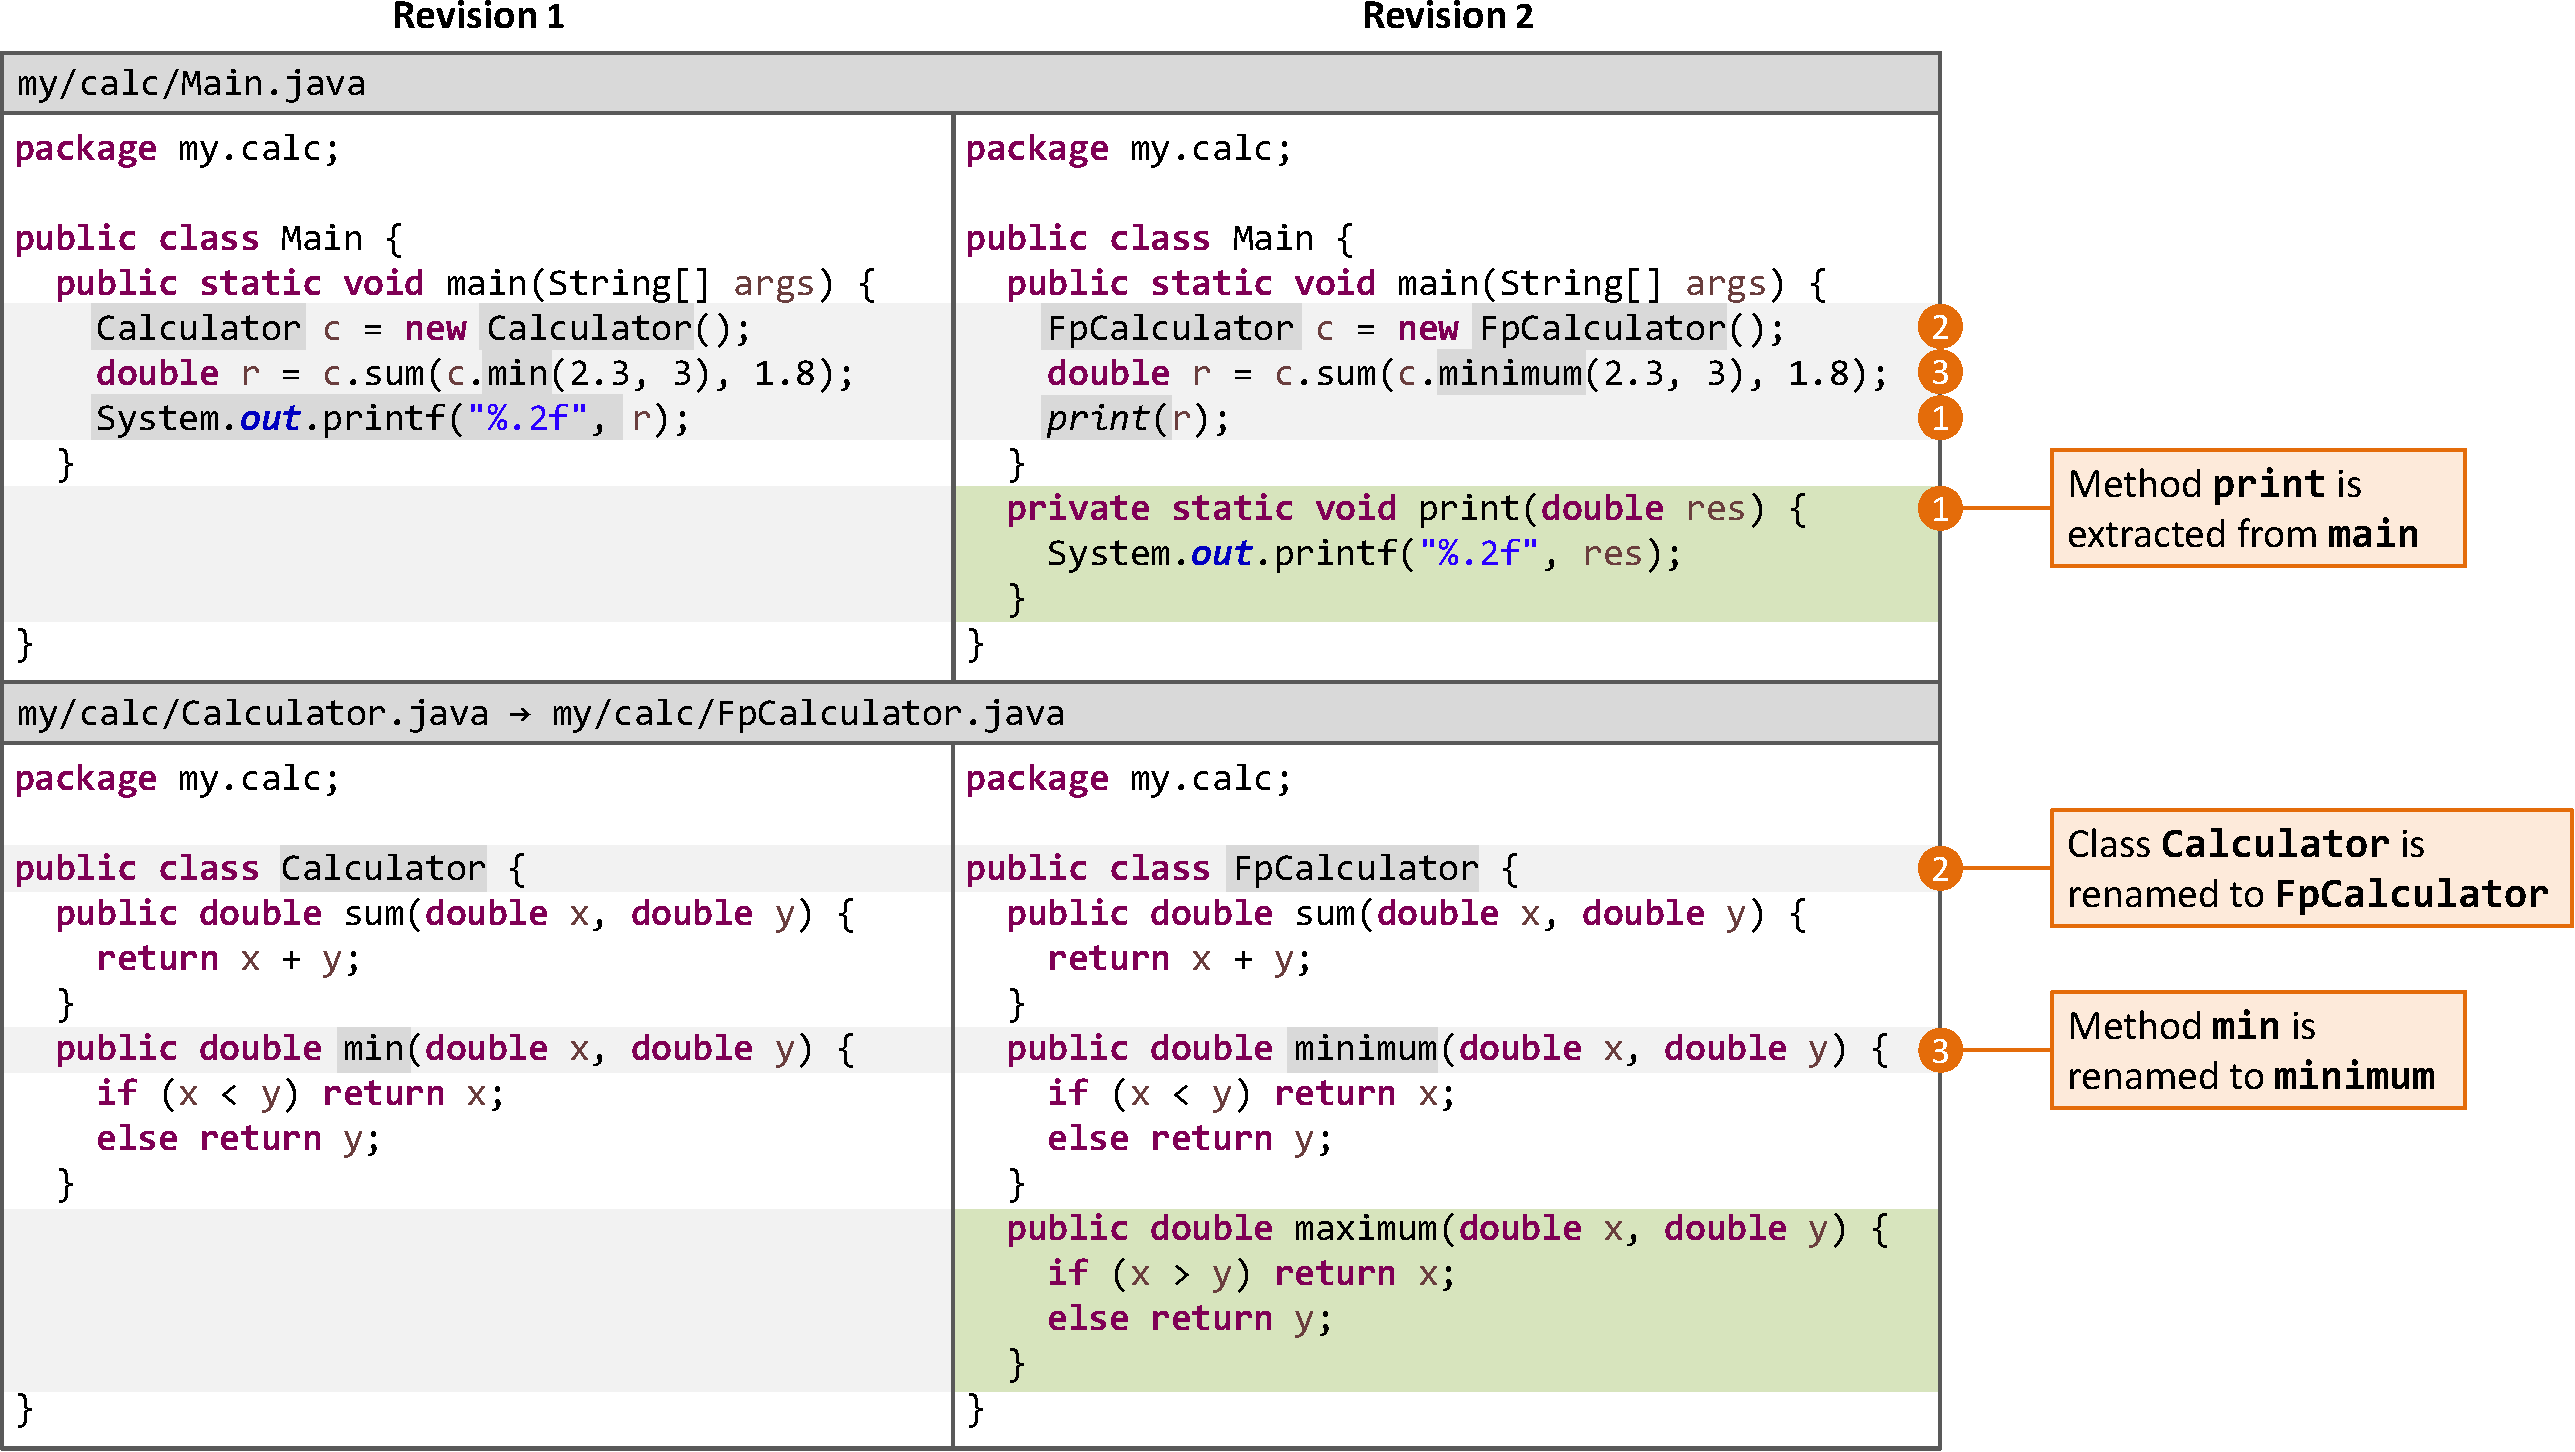
\includegraphics[width=0.9\textwidth]{img/diff1.pdf}
\caption{Illustrative diff between two revisions of a system annotated with refactoring operations}
\label{FigDiff1}
\end{figure*}


\subsection{Phase 1: Source Code Analysis}

The goal of this phase is to compute a language-independent model that represents the source code of the system, which we denote from now on as \emph{Code Structure Tree} (CST). The CST is a tree-like structure that resembles an \emph{Abstract Syntax Tree} (AST). However, in this representation we are only interested in coarse-grained code elements (e.g., classes and functions) that encompass a code region and may be referred by an identifier in other parts of the system.

To construct the CST, we need to parse the source code, generate the AST for the target programming language, and extract the necessary information.
Thus, the decision of which types of AST nodes become CST nodes depends on the programming language.
For example, in Java we represent classes, enums, interfaces, and methods as CST nodes.
In contrast, local variables are not represented.
Nevertheless, it is important to note that the granularity of the CST nodes determines the granularity of the relationships we are able to find, e.g., we can only find relationships between methods if we represent methods in the CST.
Table~\ref{TabCstNodes} lists the types of AST nodes that are represented in the CST for each programming language supported by the current implementation of our approach.

\begin{table}[htbp]
\renewcommand{\arraystretch}{1.2}
\caption{AST nodes that are represented in CSTs}
\label{TabCstNodes}
\centering
\begin{tabular}{@{}ll@{}}
\toprule
Language & Node types \\
\midrule
Java & class, enum, interface, and method \\
C & file and function \\
JavaScript & file, class, and function \\
\bottomrule
\end{tabular}
\end{table}

\begin{figure}[htb]
\centering
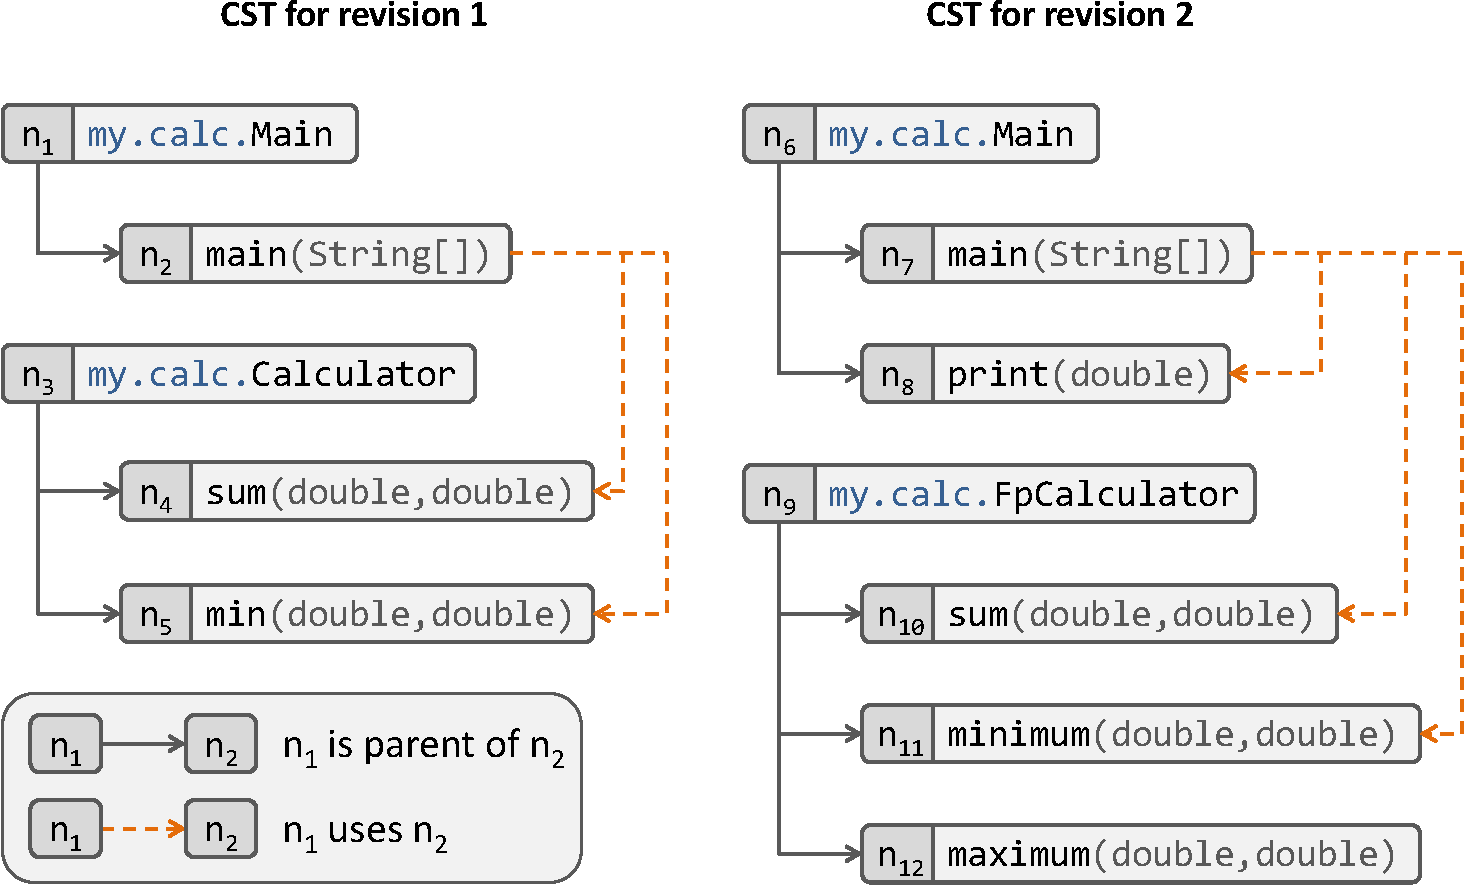
\includegraphics[width=1.0\linewidth]{img/cstDiff1.pdf}
\caption{CST of both revisions of the example system from Figure~\ref{FigDiff1}}
\label{FigJavaToCst}
\end{figure}

Figure~\ref{FigJavaToCst} exemplifies the transformation of the example system from Figure~\ref{FigDiff1} into a corresponding CST.
In revision~1, the class \codeinl{Main} is declared with a single method \codeinl{main} and the class \codeinl{Calculator} contains two methods: \codeinl{sum} and \codeinl{min}.
Note that these classes and methods become nodes in the CST for revision~1, preserving the same nesting structure of the source code. Analogously, the figure also depicts the CST for revision 2, which contains seven nodes in total (two classes and five methods).

Besides the representation of the code elements, the CST also embeds a simplified call graph and  a type hierarchy graph of the nodes within the CST, that is, there are edges to represent whether a certain node $n_1$ calls $n_2$, or whether $n_1$ is a subtype of $n_2$. The first information is necessary to find \emph{Extract} and \emph{Inline} relationships between code elements, while the second is used to find inheritance-related relationships, such as \emph{Pull Up} and \emph{Push Down}.

Moreover, along with each node of the CST, we store the following information:
\begin{description}
    \item[Identifier] \hfill \\
    An identifier of the code element in its declared scope. 
    The identifier is usually the name of the code element, but it may also contain additional information to avoid ambiguities.
    For example, the identifier of the class \codeinl{Calculator} from Figure~\ref{FigJavaToCst} is simply its name, but the identifier of the method \codeinl{sum} is \codeinl{sum(double,double)},  because there could be an overloaded method with a different signature.
    
    \item[Namespace] \hfill \\
    An optional prefix that, along with the identifier, globally identifies the code element. 
    This information only applies to root nodes and corresponds to the package or folder that the element is contained. For example, the namespace of the class \codeinl{Calculator} from Figure~\ref{FigJavaToCst} is \codeinl{my.calc.}.
    
    \item[Node type] \hfill \\
    A string that identifies the node type in the target language (class, function, method, etc.).
    
    \item[Parameters list]  \hfill \\
    An optional list of the name of the parameters, in the case the node corresponds to a method or function.
    
    \item[Tokenized source code]  \hfill \\
    The source code of the element in the form of a list of tokens.
    Here, we include all tokens in the code region that encompasses the complete declaration of the code element, including its name/signature.
    This information is necessary to compute the similarity between code elements, as explained in Section~\ref{SecCodeSim}.
    
    
    \item[Tokenized source code of the body]  \hfill \\
    The source code of the body of the code element in the form of a list of tokens.
    Here we include only the tokens within the body of the code element, but not its name/signature.
    This information is also necessary to compute the similarity between code elements in the special cases of \textit{Extract} and \textit{Inline} relationships, as explained in Section~\ref{SecSimX}.
    It is worth noting that this information is optional, as not every node has a body (e.g., abstract methods).
    
\end{description}

It is worth noting that we generate the CST only for source files that have been added, removed, or modified between revisions. 
Such information can be efficiently obtained from version control systems, without the need to analyze the content of all files within the repository.
This way, we avoid a costly operation that might compromise the scalability of our approach, as large repositories contain thousands of source files, but only a small fraction of them change between revisions.

Although the construction of the CST is a language-specific process, from this point on, the approach is language-independent and relies only on information encoded in CSTs.
This way, one is able to extend our approach to work with different programming languages only by implementing the \emph{Source Code Analysis} module.
To demonstrate this capability, we provide implementations for three programming languages: Java, C, and JavaScript.\footnote{\url{https://github.com/aserg-ufmg/RefDiff}}


\subsection{Phase 2: Relationship Analysis}

This phase takes as input the CST's of revisions $v_1$ and $v_2$ and outputs the set of relationships $R$. Let $N_1$ and $N_2$ be the sets of code elements from the CST's of $v_1$ and $v_2$ respectively. Each relationship $r \in R$ is a triple $(n_1, n_2, t)$, where $n_1 \in N_1$, $n_2 \in N_2$, and $t$ is a relationship type. The types of relationships are listed in the first column of Table~\ref{TabRelationshipTypes}, and can be subdivided into two groups:
\begin{itemize}
\item \textbf{Matching relationships}, which indicate that the node $n_1$ corresponds to $n_2$ in the subsequent revision.
The possible matching relationships are \textit{Same}, \textit{Convert Type}, \textit{Pull Up}, \textit{Push Down}, \textit{Change Signature}, \textit{Move}, \textit{Rename}, and \textit{Move and Rename}.
We say that a node $n_1$ matches with $n_2$ if exists a relationship $(n_1, n_2, t) \in R$ such that $t$ is a matching relationship.

\item \textbf{Non-matching relationships}, which indicate that either node $n_1$ is decomposed to create $n_2$, or node $n_1$ is incorporated into $n_2$.
There are four non-matching relationships: \textit{Extract Supertype}, \textit{Extract}, \textit{Extract and Move}, and \textit{Inline}.
\end{itemize}


\subsubsection{General algorithm to find relationships}

\begin{figure}[htbp]
\small
\begin{algorithmic}[1]
\Procedure{FindRelationships}{$t_1,t_2$}
\State $R \gets \emptyset$
\State $M \gets \emptyset$
\State $\textsc{findMatchingsById}(t_1,t_2)$
\State $\textsc{findMatchingsBySim}$
\State $\textsc{findMatchingsByChildr}$
\State $\textsc{resolveMatchings}$
\State $\textsc{findNonMatchingRel}$
\State \Return $R$
\\
\Procedure{findMatchingsById}{$p_1,p_2$}
\ForEach{$(n_1, n_2) \in \rdchildren(p_1) \times \rdchildren(p_2)$}
  \If {$\rdsig(n_1) = \rdsig(n_2) \land \rdns(n_1) = \rdns(n_2)$}
    \State $\textsc{addMatch}(n_1, n_2)$
  \EndIf
\EndFor
\EndProcedure
\\
\Procedure{findMatchingsBySim}{}
\ForEach{$(n_1, n_2) \in \rdsortbysim(N^- \times N^+)$}
  \If {$\mathit{findMatchRel}(n_1, n_2) \neq \emptyset$}
    \State $\textsc{addMatch}(n_1, n_2)$
  \EndIf  
\EndFor
\EndProcedure
\\
\Procedure{findMatchingsByChildr}{}
\ForEach{$(n_1, n_2) \in \rdsortbysim(N^- \times N^+)$}
  \If {$\mathit{matchingChildr}(n_1, n_2) > 1\,\land \newline
    \hspace*{5.5em} \rdnsim(n_1, n_2) > 0.5$}
    \State $\textsc{addMatch}(n_1, n_2)$
  \EndIf
\EndFor
\EndProcedure
\\
\Procedure{resolveMatchings}{}
\ForEach{$(n_1, n_2) \in M$}
  \State $R \gets R \cup \mathit{findMatchRel}(n_1, n_2)$
\EndFor
\EndProcedure
\\
\Procedure{findNonMatchingRel}{}
\ForEach{$(n_1, n_2) \in M_1 \times N^+$}
  \State $R \gets R \cup \mathit{findExtractSupertype}(n_1, n_2)$
  \State $R \gets R \cup \mathit{findExtract}(n_1, n_2)$
  \State $R \gets R \cup \mathit{findExtractMove}(n_1, n_2)$
\EndFor
\ForEach{$(n_1, n_2) \in N^- \times M_2$}
  \State $R \gets R \cup \mathit{findInline}(n_1, n_2)$
\EndFor
\EndProcedure
\\
\Procedure{addMatch}{$n_1, n_2$}
\If {$n_1 \in N^- \land n_2 \in N^+$}
  \State $M \gets M \cup \{(n_1, n_2)\}$
  \State $\textsc{findMatchingsById}(n_1,n_2)$
\EndIf
\EndProcedure
\\
\EndProcedure
\end{algorithmic}
%\vspace{1em}
%{
%\footnotesize
%\renewcommand{\arraystretch}{1.3}
%\begin{tabular}{@{}ll@{}}
%\midrule
%\multicolumn{2}{c}{\textbf{Definitions}}\\
%$\rdchildren(n)$ & set of children of $n$ in the CST\\
%$\rdsortbysim(S)$ & elements of $S$ sorted by $\rdsim$ function descending\\
%\midrule
%\end{tabular}
%}
\caption{Algorithm to find relationships}
\label{AlgoGeneral}
\end{figure}






Our approach employs the algorithm described in Figure~\ref{AlgoGeneral} to find the relationships (i.e., to compute the set $R$).
The procedure \textsc{FindRelationships} has two parameters, $t_1$ and $t_2$, which are the root nodes of the CST's of both revisions.
Initially, we define $R \gets \emptyset$ as the set of relationships found so far (line~2).
Additionally, we also define $M \gets \emptyset$ as the set of pairs of matching nodes found so far (line~3).
Then, we execute four subroutines:
\begin{enumerate}

\item In \textsc{findMatchingsById}, we recursively look for matching nodes that have the same identifier and parent, i.e., we assume that code elements with the same identifier and parent are the same.
Such assumption allows us to match many code elements at this step, reducing the number of possibilities that need to be checked in the next steps.
The procedure consists of a loop that pairs the children of the nodes received as arguments and calls the procedure \textsc{addMatch} whenever a matching is found (line~13).
On its turn, \textsc{addMatch} (lines 46-51) adds a pair of matching nodes to $M$ and calls \textsc{findMatchingsById} again to look for matchings on their children, completing the recursion.
The matching pairs found in this step will be resolved to \textit{Same} and \textit{Convert type} relationships later (see step~4).

\item In \textsc{findMatchingsBySim}, we look for matching nodes based on code similarity.
The goal is to find \textit{Change Signature}, \textit{Pull Up}, \textit{Push Down}, \textit{Move}, \textit{Rename}, and \textit{Move and Rename} relationships.
%The procedure starts by computing the set $M'$, which contains unmatched pairs of nodes from $t_1$ and $t_2$.
The procedure iterates over the unmatched pairs of nodes sorted by similarity in descending order.
We use the notation $N^-$ to denote the set of unmatched nodes from $t_1$ (presumably deleted) and $N^+$ to denote the set of unmatched nodes from $t_2$ (presumably added).
For each pair $(n_1, n_2)$, the procedure checks if it meets the conditions (specified in the second column of Table~\ref{TabRelationshipTypes}) for any matching relationship by calling $\mathit{findMatchRel}(n_1, n_2)$.
%Then, it repeatedly takes a pair $(n_1, n_2)$ from $M'$, sorting by the $\rdrank$ function, and checks if it meets the conditions (specified in the second column of Table~\ref{TabRelationshipTypes}) for any matching relationship by calling $\mathit{findMatchRel}(n_1, n_2)$.
This function returns a singleton containing a matching relationship or an empty set if none of the conditions are met.
Last, the \textsc{addMatch} subroutine is called in the case of a matching (line~24).
The conditions to find those relationships and the $\rdsortbysim$ function rely on a code similarity metric, which is described in details in Section~\ref{SecCodeSim}.

\item In \textsc{findMatchingsByChildr}, we look for matching nodes based on matchings of their children and name similarity. 
Once again, the procedure iterates over the unmatched pairs of nodes sorted by similarity in descending order.
For each pair $(n_1, n_2)$, if $n_1$ has more than one children that match with $n_2$'s children and their names are similar, then we consider it a match. The $\rdnsim$ function, used to compute the similarity between names, is described in details in Section~\ref{SecNameSim}.
This heuristic is intended to cover the cases when a code element (e.g., a class) is moved (and/or renamed) and it is also subjected to many additions or removals of its members, so that its similarity with its matching pair is not enough to yield a match in the previous step.
Failing to detect that a class has been moved (or renamed) may yield several incorrect \textit{Move} relationships between its members before and after the change.


\item In \textsc{resolveMatchings}, we add the relationships corresponding to the matching pairs found at steps~1, 2, and 3 to $R$.
The procedure iterates over the elements of $M$ and calls $\mathit{findMatchRel}$ to find which relationship type holds between $n_1$ and $n_2$ (according to the conditions defined in Table~\ref{TabRelationshipTypes}).
By the end of this step, $R$ contains all matching relationships found.
The rationale for postponing the resolution of the relationship type is discussed in Section~\ref{SecDependentConflictingRel}.

\item In \textsc{findNonMatchingRel}, we look for non-matching relationships.
First, we iterate over the pairs of matched/unmatched nodes, i.e., $M_1 \times N^+$, to look for \textit{Extract Supertype}, \textit{Extract} and \textit{Extract and Move} relationships.
Similarly, we also iterate over the pairs of unmatched/matched nodes ($N^- \times M_2$) to look for \textit{Inline} relationships.
The functions $findExtractSupertype$, $findExtract$, $findExtractMove$, and $findInline$ check the  preconditions for the corresponding relationship types, according to Table~\ref{TabRelationshipTypes}.
After this last step, $R$ contains all matching and non-matching relationships between CST nodes of both revisions.
\end{enumerate}


\begin{table*}[htbp]
\renewcommand{\arraystretch}{1.3}
\caption{Definitions used in the Algorithm from Figure~\ref{AlgoGeneral} and in the conditions from Table~\ref{TabRelationshipTypes}}
\label{TabDefinitions}
\centering
\begin{tabular}{@{}lll@{}}
\toprule
%\multicolumn{3}{c}{\textbf{Definitions}}\\
\begin{tabular}{@{}ll@{}}
$M_1$ & the set of nodes from $N_1$ that matches with a node from $N_2$\\
$M_2$ & the set of nodes from $N_2$ that matches with a node from $N_1$\\
$N^-$ & the set of unmatched nodes from $N_1$ ($N_1 \setminus M_1$)\\
$N^+$ & the set of unmatched nodes from $N_2$ ($N_2 \setminus M_2$)\\
$n'$ & the code element that matches with $n$ in the other revision\\
$\rdparent(n)$ & parent of a node $n$ (it may be a namespace or a CST node)\\
$\rdns(n)$ & namespace of the code element $n$\\
$\rdchildren(n)$ & set of children of $n$ in the CST\\
\end{tabular}
& &
\begin{tabular}{@{}ll@{}}
$\rdname(n)$ & simple name of the code element $n$\\
$\rdsig(n)$ & identifier of the code element $n$\\
$\rdtype(n)$ & node type of the code element $n$\\
$\rdsub(n_1, n_2)$ & $n_1$ is subtype of $n_2$\\
$\rduses(n_1, n_2)$ & $n_1$ uses $n_2$\\
$\rdsim(n_1, n_2)$ & code similarity between $n_1$ and $n_2$\\
$\rdnsim(n_1, n_2)$ & name similarity between $n_1$ and $n_2$\\
$\rdsimx(n_1, n_2)$ & extract similarity between $n_1$ and $n_2$\\
$\rdsortbysim(S)$ & elements of $S$ sorted by $\rdsim$ descending\\
\end{tabular}
\\
\bottomrule
\end{tabular}

\end{table*}



\begin{table*}[htbp]
\renewcommand{\arraystretch}{1.3}
\caption{Relationship types and the conditions to find them}
\label{TabRelationshipTypes}
\centering
\begin{tabular}{@{}lll@{}}
\toprule
Relationship type & \multicolumn{2}{l}{Conditions} \\
\midrule
& \multicolumn{2}{l}{$(n_1, n_2) \in N^- \times N^+$, such that:}\\
Same & & $\rdtype(n_1) = \rdtype(n_2) \land \rdsig(n_1) = \rdsig(n_2) \land \rdparent(n_1)' = \rdparent(n_2)$ \\
Convert Type & & $\rdtype(n_1) \neq \rdtype(n_2) \land \rdsig(n_1) = \rdsig(n_2) \land \rdparent(n_1)' = \rdparent(n_2)$ \\
Pull Up & & $\rdtype(n_1) = \rdtype(n_2) \land \rdsig(n_1) = \rdsig(n_2) \land \rdsub(\rdparent(n_1)', \rdparent(n_2))$ \\
Push Down & & $\rdtype(n_1) = \rdtype(n_2) \land \rdsig(n_1) = \rdsig(n_2) \land \rdsub(\rdparent(n_2), \rdparent(n_1)')$ \\
Change Signature & & $\rdtype(n_1) = \rdtype(n_2) \land \rdsig(n_1) \neq \rdsig(n_2) \land \rdname(n_1) = \rdname(n_2) \land \rdparent(n_1)' = \rdparent(n_2) \land \rdsim(n_1, n_2) > 0.5$ \\
Move & & $\rdtype(n_1) = \rdtype(n_2) \land \rdname(n_1) = \rdname(n_2) \land \rdparent(n_1)' \neq \rdparent(n_2) \land \rdsim(n_1, n_2) > 0.5$ \\
Rename & & $\rdtype(n_1) = \rdtype(n_2) \land \rdname(n_1) \neq \rdname(n_2) \land \rdparent(n_1)' = \rdparent(n_2) \land \rdsim(n_1, n_2) > 0.5$ \\
Move and Rename & & $\rdtype(n_1) = \rdtype(n_2) \land \rdname(n_1) \neq \rdname(n_2) \land \rdparent(n_1)' \neq \rdparent(n_2) \land \rdsim(n_1, n_2) > 0.5$ \\
\addlinespace
& \multicolumn{2}{l}{$(n_1, n_2) \in M_1 \times N^+$, such that:}\\
Extract Supertype & & $\exists (n_3, n_4, \mathit{PullUp}) \in R\, (n_1 = \rdparent(n_3) \land n_2 = \rdparent(n_4))$ \\
Extract & & $\rduses(n_1', n_2) \land \rdparent(n_1)' = \rdparent(n_2) \land \rdsimx(n_2, n_1) > 0.5$ \\
Extract and Move & & $\rduses(n_1', n_2) \land \rdparent(n_1)' \neq \rdparent(n_2) \land \rdsimx(n_2, n_1) > 0.5$ \\
\addlinespace
& \multicolumn{2}{l}{$(n_1, n_2) \in N^- \times M_2$, such that:}\\
Inline & & $\rduses(n_1, n_2') \land \rdsimx(n_1, n_2) > 0.5$ \\
\bottomrule
\end{tabular}
\end{table*}







Figure~\ref{FigRelationships1} shows the relationships we find after running RefDiff in the example system from Figure~\ref{FigDiff1}.
Each relationship is represented by an edge connecting nodes from the left and right CSTs.
There are three relationships of the type \textit{Same}, involving the code elements whose identifiers do not change: the class \codeinl{Main} and the methods \codeinl{main} and \codeinl{sum}.
Two of the relationships are of type \textit{Rename}, indicating that the class \codeinl{Calculator} is renamed to \codeinl{FpCalculator}, and the method \codeinl{min} is renamed to \codeinl{minimum}.
Moreover, there is an \textit{Extract} relationship indicating that the method \codeinl{print} is extracted from \codeinl{main}.
Finally, we can also note that two nodes, $n_8$ and $n_{12}$, are not involved in matching relationships. Thus, we classify them as added code elements.
In this example, as every node on the left side is matched, there are no deleted code elements.


\begin{figure}[htbp]
\centering
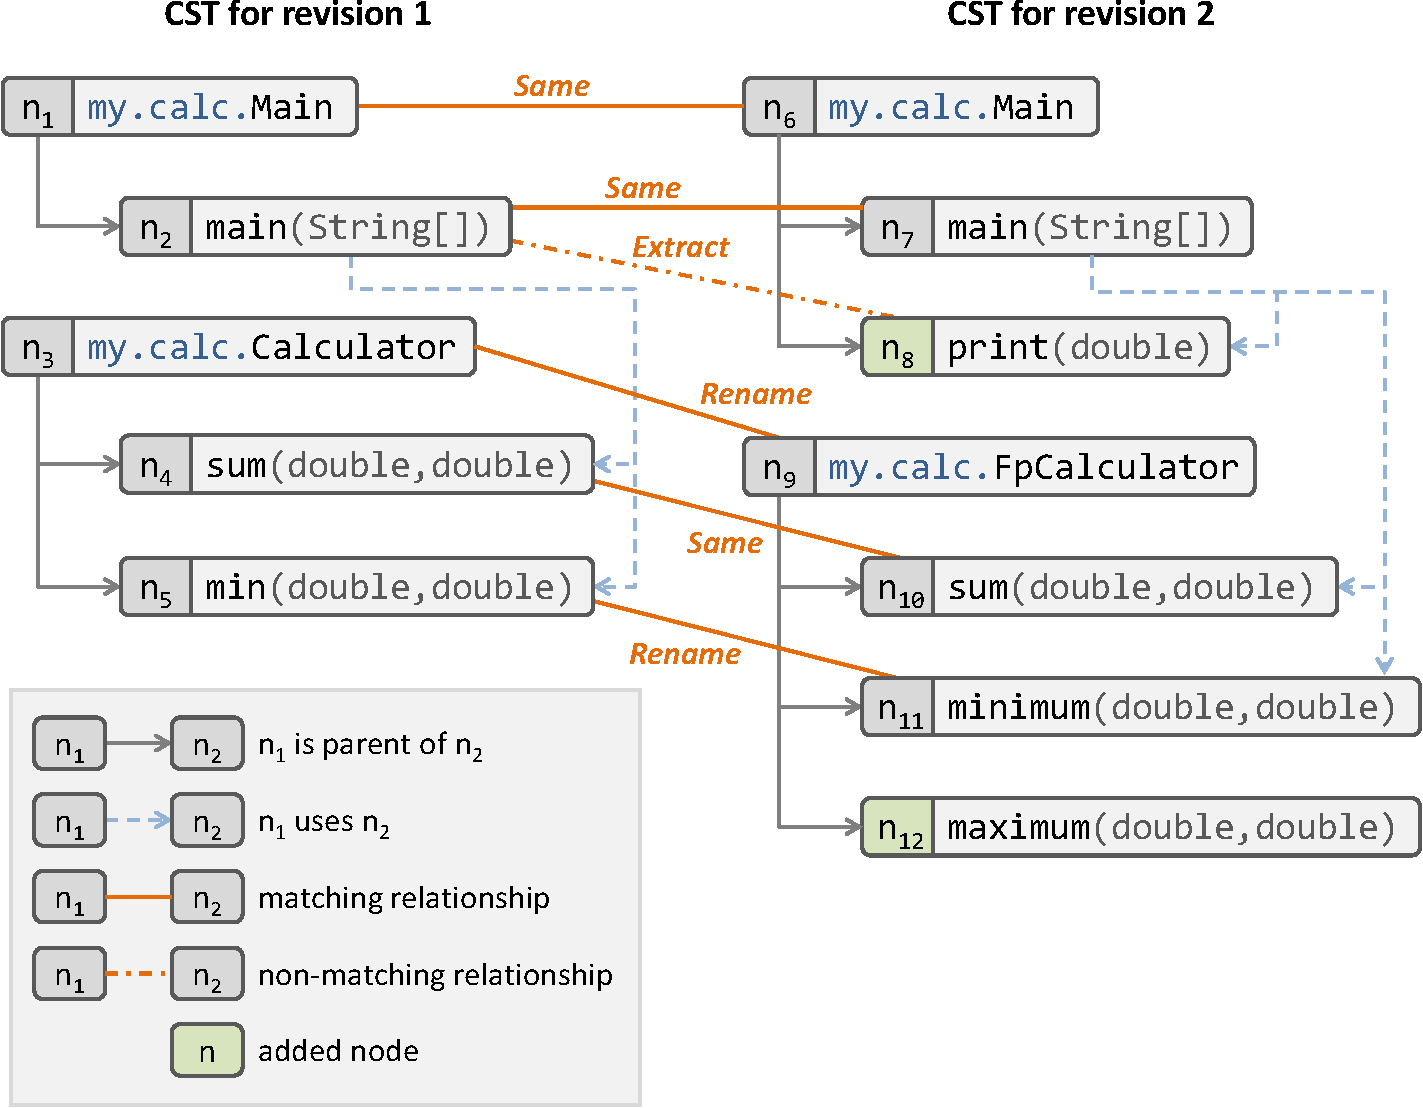
\includegraphics[width=1.0\linewidth]{img/relationshipDiff1.pdf}
\caption{Relationships found in the example from Figure~\ref{FigDiff1}}
\label{FigRelationships1}
\end{figure}


\subsubsection{Dependent and conflicting relationships}
\label{SecDependentConflictingRel}

In some cases, correctly finding a relationship depends on finding a prior relationship.
For example, consider the relationship $(n_5, n_{11}, Rename)$ in Figure~\ref{FigRelationships1} (method \codeinl{min} renamed to \codeinl{minimum}).
The conditions for this relationship includes the clause $\rdparent(n_5)' = \rdparent(n_{11})$, which means that the matching node of the parent of $n_5$ should be equal to the parent of $n_{11}$ (see Table~\ref{TabRelationshipTypes}, \textit{Rename} row).
This clause only yields true after the matching pair $(n_3, n_9)$ is added to $M$, i.e., after we find out that \codeinl{Calculator} is renamed to \codeinl{FpCalculator}.
In fact, if we call $\mathit{findMatchRel}(n_5, n_{11})$ before $M$ contains $(n_3, n_9)$, we would incorrectly classify it as a \textit{Move and Rename} relationship.
To address this issue, we only resolve the actual relationship types in steps~4 and~5, after all matching pairs are found (note that in steps~1, 2, and 3 we record the matching pairs in $M$, purposely ignoring the type of relationship).
%Moreover, non-matching relationships, which also depends on the matchings found, are analyzed in the last step. 

Another issue which we may face when looking for relationships are conflicts, i.e., two or more matching relationships hold for the same code element (according to conditions from Table~\ref{TabRelationshipTypes}).
For instance, in the example from Figure~\ref{FigRelationships1}, the conditions for \textit{Rename} yield true for the pair of methods \codeinl{min} and \codeinl{minimum} because their source code are similar and their parents match.
However, this is also the case for the pair of methods \codeinl{min} and \codeinl{maximum}, whose bodies are also similar.
We cannot match the same node twice, thus, we must decide upon which relationship we will accept and discard the other one.
This issue is addressed in the \textsc{findMatchingsBySim} procedure by using the $\rdrank$ function to sort the potential matching pairs, enforcing that we take first the most likely matches.
The $\rdrank$ function relies on a similarity metric, which we discuss in details in Section~\ref{SecCodeSim}.
After a matching pair $(n_1, n_2)$ is added to $M$, no more matchings involving $n_1$ or $n_2$ are accepted, because \textsc{addMatch} procedure checks that $n_1 \in N^- \land n_2 \in N^+$ (line~47).







\subsection{Code Similarity}
\label{SecCodeSim}

\begin{figure*}[htb]
\renewcommand{\arraystretch}{1.3}
\centering
\footnotesize
\begin{tabular}{@{}llll@{}}
\begin{tabular}{p{6.5cm}}
\multicolumn{1}{c}{\textbf{Source code of a class}} \\
\begin{lstlisting}
public class Calculator {

  public int sum(int x, int y) {
    return x + y;
  }

  public int min(int x, int y) {
    if (x < y) return x;
    else return y;
  }

  public double power(int b, int e) {
    return Math.pow(b, e);
  }
}
\end{lstlisting}\\

\end{tabular}
& {\Large $\Rightarrow$} &
\begin{tabular}{|l|r|r|r|}
\multicolumn{4}{c}{\textbf{Multiset of tokens for each method}} \\
\hline
Token $t$ & $m_{\mathtt{sum}}(t)$ & $m_{\mathtt{min}}(t)$ & $m_{\mathtt{power}}(t)$\\
\hline
\codeinl{return} & 1 & 2 & 1 \\
\codeinl{x}      & 1 & 2 & 0 \\
\codeinl{+}      & 1 & 0 & 0 \\
\codeinl{y}      & 1 & 2 & 0 \\
\codeinl{;}      & 1 & 2 & 1 \\
\codeinl{if}     & 0 & 1 & 0 \\
\codeinl{(}      & 0 & 1 & 1 \\
\codeinl{<}      & 0 & 1 & 0 \\
\codeinl{)}      & 0 & 1 & 1 \\
\codeinl{else}   & 0 & 1 & 0 \\
\codeinl{Math}   & 0 & 0 & 1 \\
\codeinl{.}      & 0 & 0 & 1 \\
\codeinl{pow}    & 0 & 0 & 1 \\
\codeinl{b}      & 0 & 0 & 1 \\
\codeinl{,}      & 0 & 0 & 1 \\
\codeinl{e}      & 0 & 0 & 1 \\
\hline
\end{tabular} &
\begin{tabular}{|r|}
\multicolumn{1}{c}{} \\
\hline
$n_t$\\
\hline
3 \\
2 \\
1 \\
2 \\
3 \\
1 \\
2 \\
1 \\
2 \\
1 \\
1 \\
1 \\
1 \\
1 \\
1 \\
1 \\
\hline
\end{tabular}
\end{tabular}
\caption{Transformation of the body of methods into a multiset of tokens}
\label{FigSourceCodeTransformation}
\end{figure*}

A key element of our approach to find relationships, as previously mentioned, is computing the similarity between code elements (i.e., CST nodes).
The first step to compute this similarity is to represent their source code as a multiset (or bag) of tokens.
A multiset is a generalization of the concept of a set, but it allows multiple instances of the same element.
The multiplicity of an element is the number of occurrences of that element within the multiset. Formally, a multiset can be defined in terms of a multiplicity function $m: U \to \mathbb{N}$, where $U$ is the set of all possible elements. In other words, $m(t)$ is the multiplicity of the element $t$ in the multiset. Note that the multiplicity of an element that is not in the multiset is zero.

For example, Figure~\ref{FigSourceCodeTransformation} depicts the transformation of the source code of three methods (\codeinl{sum}, \codeinl{min}, and \codeinl{power}), of the class \codeinl{Calculator}, into multisets of tokens. In this figure, the multiplicity function $m$ for each method is represented in a tabular form. For example, the multiplicity of the token \codeinl{y} in method \codeinl{min} is two (i.e., $m_{\mathtt{min}}(\mathtt{y}) = 2$), whilst the multiplicity of the token \codeinl{if} in method \codeinl{power} is zero (i.e., $m_{\mathtt{power}}(\mathtt{if}) = 0$).

After extracting a multiset of tokens, we also compute a weight for each token
of the source code.
In fact, some tokens are more important than others to discriminate a code element.
For example, in Figure~\ref{FigSourceCodeTransformation}, all three methods contain the token \codeinl{return}. In contrast, only one method (\codeinl{power}) contains the token \codeinl{Math}. Therefore, the later is a better indicator of similarity between methods than the former.

In order to take this into account, we employ a variation of the TF-IDF weighting scheme~\cite{salton1986introduction}, which is a well-known technique from information retrieval.
TF-IDF, which is the short form of \emph{Term Frequency–Inverse Document Frequency}, reflects how important a term is to a document within a collection of documents.
In the context of code elements, we consider a token as a term, and a code element as a document.
Let $E$ be the set of all code elements and $n_t$ be the number of elements in $E$ that contains the token $t$. The Inverse Document Frequency ($\mathit{idf}$), is defined as:
\begin{align}
\mathit{idf}(t) = \log (1 + \frac{|E|}{n_t})
\end{align}

Note that the value of $\mathit{idf}(t)$ decreases as $n_t$ increases, because the more frequent a token is among the collection of code elements, the less important it is to distinguish them.
For example, in Figure~\ref{FigSourceCodeTransformation}, the token \codeinl{y} occurs in two methods (\codeinl{sum} and \codeinl{min}). Thus, its $\mathit{idf}$ is:

\[
\mathit{idf}(\mathtt{y}) = 
\log (1 + \frac{|E|}{n_t}) = 
\log (1 + \frac{3}{2}) = 0.398
\]

On the other hand, the token \codeinl{else} occurs in one method ($\mathtt{min}$), and therefore its $\mathit{idf}$ is:

\[
\mathit{idf}(\mathtt{else}) = 
\log (1 + \frac{|E|}{n_t}) = 
\log (1 + \frac{3}{1}) = 0.602
\]

Last, to compute the similarity between two code elements $e_1$ and $e_2$, we use a generalization of the Jaccard coefficient, known as weighted Jaccard coefficient~\cite{chierichetti2010finding}.
Let $U$ be the set of all possible tokens and $m_i: U \to \mathbb{N}$ be the multiplicity function representing the multiset of tokens of a code element $e_i$.
We define the similarity between $e_1$ and $e_2$ by the following formula:


\begin{align}
\label{WJaccard}
\rdsim(e_1, e_2) = \frac{\sum_{t \in U} \min(m_1(t), m_2(t)) \times \mathit{idf}(t) }
                        {\sum_{t \in U} \max(m_1(t), m_2(t)) \times \mathit{idf}(t) }
\end{align}

The rationale behind this formula is that the similarity is at maximum (1.0) when the multiset of tokens representing $e_1$ and $e_2$ contain the same tokens with the same cardinality. In contrast, if the multisets contain no tokens in common, the similarity is zero. Additionaly, tokens with higher $\mathit{idf}$ will have a higher weight.
%It is worth noting that when both multisets are empty, the denominator of the formula is zero, which yields undefined. We handle such special case considering that the similarity is zero.


\subsubsection{Name similarity}
\label{SecNameSim}

Besides relying on the code similarity, our algorithm also depends on the function $\rdnsim(n_1, n_2)$ in Step~3.
This function denotes the similarity between the names of the code elements $n_1$ and $n_2$.
For computing $\rdnsim$, we first decompose the identifiers of $n_1$ and $n_2$ into their composing words. Specifically, we split camel case (e.g., \codeinl{myIdentifier}) or snake case patterns (e.g., \codeinl{my\_identifier}) . For example, \codeinl{SomeLong\_Name} yields three terms: \codeinl{Some}, \codeinl{Long}, and \codeinl{Name}.
Then, we compute $\rdnsim$ using the same formula from $\rdsim$ (see Equation~\ref{WJaccard}), but in this case, each multiset of tokens contains the terms composing the identifiers of $n_1$ and $n_2$.


\subsubsection{Extract similarity}
\label{SecSimX}

While the similarity function $\rdsim$ presented previously is suitable to compute whether two code elements are similar, it is not appropriate to assess whether a code element is extracted from another one, because their source code may be significantly different on their entirety.
However, if a method $e_2$ is extracted from $e_1$, we expect that part of the code of $e_1$ is moved to $e_2$.
Therefore, the source code of the body of $e_2$ should be similar to the source code removed from $e_1$.
Additionally, not all code removed from $e_1$ may have been moved to $e_2$, i.e., some parts of the code may have been extracted to other locations or simply deleted.
To be less susceptible to this issue, our similarity index for \textit{Extract} relationships rely on the following assumption: the code from the body of $e_2$ should be mostly contained in the code removed from $e_1$.

%However, we face two issues when directly comparing the code removed from $e_1$ with the body of $e_2$. First, not all code removed from $e_1$ may have been moved to $e_2$, i.e., some parts of the code may have been extracted to other locations or simply deleted. Second, $e_2$ may contain additional code, introduced after the extraction. In fact, one of the common reasons to extract a method/function is to facilitate the addition of new code~\cite{fse2016-why-we-refactor}. Thus, to be less susceptible to those issues, our similarity index for \textit{Extract} relationships relies on two heuristics: (i) the code from the body of $e_2$ should be mostly contained in the code removed from $e_1$, or (ii) the code removed from $e_1$ should be mostly contained in the body of $e_2$.

Thus, to compute the extract similarity, first we need to compute the code removed from $e_1$. As we represent the source code as multisets of tokens, we are able to use the subtract operation to achieve this goal.
Let $m_1$ be the multiset of tokens of $e_1$ before the change and $m_1'$ be the multiset of tokens of $e_1$ after the change.
The subtract operation between both multisets, which we denote by $m_1' \setminus m_1$, yields a new multiset $m_1^-$ defined by the following multiplicity function:
\begin{align}
m_1^-(t) = \max(0, m_1'(t) - m_1(t))
\end{align}

Besides computing the code removed from $e_1$, we need to measure if its contained within $e_2$. Thus, we employ a variation of the weighted Jaccard coefficient introduced previously (see Equation~\ref{WJaccard}), which is defined as:
\begin{align}
\rdsimc(m_1, m_2) = \frac{\sum_{t \in U} \min(m_1(t), m_2(t)) \times \mathit{idf}(t)}
                        {\sum_{t \in U} m_1(t) \times \mathit{idf}(t)}
\end{align}
where $m_1$ and $m_2$ are multisets (defined by their multiplicity functions).
In this variation, we change the denominator of Equation~\ref{WJaccard} to include only the multiplicity of the tokens from the first multiset (not their union).
This way, the similarity is at maximum (1.0) when $m_1$ is a subset of $m_2$, even if both multisets are not identical. In contrast, the similarity is zero when the intersection between $m_1$ and $m_2$ is empty.


Given these definitions, we are able to define the extract similarity index, $\rdsimx$, as:
\begin{align}
%\rdsimx(e_1, e_2) = \max( \rdsimc(m_1^-, m_2), \rdsimc(m_2, m_1^-) )
\rdsimx(e_1, e_2) = \rdsimc(m_2, m_1^-)
\end{align}
where $m_1^-$ is the multiset representing the code removed from $e_1$ ($m_1 \setminus m_1'$) and $m_2$ is the multiset representing the source code of the body of $e_2$.
The rationale behind this formula is that the similarity is at maximum
%when $m_1^-$ is a subset of $m_2$, or 
when $m_2$ is a subset of $m_1^-$, addressing the previously described heuristic.
%that the code from the body of $e_2$ should be mostly contained in the code removed from $e_1$.



%When building the multiset of tokens representing the source code of the body of a code element, we ignore any occurrence of identifiers that are parameters. 


\subsubsection{Inline similarity}
\label{SecSimI}

The similarity index for computing \textit{Inline} relationships is analogous to the \textit{Extract} similarity index.
%, but we adopt a simpler heuristic in this instance because it is less common to introduce code changes in the inlined method along with the refactoring operation \todo{esta explicacao nao tem muito fundamento na verdade}.
If a code element $e_1$ is inlined into a code element $e_2$, we expect that the code from the body of $e_1$ should be mostly contained in the code added to $e_2$. Specifically, we define the inline similarity index, $\rdsimi$, as:
\begin{align}
\rdsimi(e_1, e_2) = \rdsimc(m_1, m_2^+)
\end{align}
where $m_1$ is the multiset representing the source code of the body of $e_1$ and $m_2^+$ is the multiset representing the code added to $e_2$ ($m_2' \setminus m_2$). Such similarity index is at maximum (1.0) when $m_1$ is a subset of the added code ($m_2^+$).





\subsubsection{Ignoring parameters and return keywords}

%\noindent\textbf{Ignoring parameters and \codeinl{return} keywords}\\
When retrieving the tokenized source code of the body of a code element, some tokens are ignored to avoid that syntactical constructs necessary to its declaration
introduce noise when computing the \textit{Extract} or \textit{Inline} similarity index.
For example, let's take the refactoring operation \#1 depicted in Figure~\ref{FigDiff1}: \codeinl{print} is extracted from \codeinl{main}.
The body of the new method \codeinl{print} contains a single statement:
\begin{lstlisting}
System.out.printf("%.2f", res);
\end{lstlisting}
All the tokens within this method are present in \codeinl{main} before the extraction, except the identifier \codeinl{res}, which is a declared parameter of \codeinl{print}. In fact, in the original statement, a variable \codeinl{r} is used in place of \codeinl{res}. To be less susceptible to such differences, we omit all occurences of parameters in the tokenized source code of the body. Similarly, occurences of \codeinl{return} keywords are also ignored because they may be introduced when turning the extracted code into a method.
It is worth noting that the filtering such tokens is of responsability of the source analysis module. Thus, specific rules may be implemented according to the peculiarities of the programming language.

\section{Evaluation}

\subsection{Evaluation Procedure}

\subsection{Java}

To evaluate the performance of RefDiff in Java we initially use an oracle proposed by Tsantalis et al.~\cite{xx}. This oracle includes 3,188 manually-validated refactoring instances, detected in 185 open source projects, and covering 15 refactoring operations. \todo{discutir quais sao cobertos ou nao por RefDiff 2.0}. We also use this oracle to compare RefDiff's precision and recall against RefactoringMiner, a state-of-the-art tool for detecting refactorings in Java.

First, we run RefDiff on the oracle commits. For each commit with a detected refactoring $r$ we checked whether $r$ is in the oracle. If yes, $r$ is a true positive; otherwise, $r$ was evaluated by two authors of this paper, to check whether it is a true positive or not. This extra manual validation is needed because the initial oracle must not be granted as complete, i.e., including all refactorings performed in the set of analysed commits. In reality, this oracle was constructed based on an initial list of refactorings produced by RefactoringMiner and RefDiff 1.0. For this reason, it might miss true refactorings only detected by the improved implementation of RefDiff, described in this paper.

After following this procedure, RefDiff 2.0 detected 406 new refactoring instances (i.e., not listed in the initial oracle), which were  validated by two paper's authors, called here validators.  In the case of 269 refactorings (66\%), the validators agreed on their classification, including 184 refactorings labelled as true positives by both validators and 85 labelled as false positives. After this initial and independent validation, the validators discussed together the remaining 137 cases (34\%), to reach an agreement. As a result, xx refactorings were considered true positives and xx refactorings were classified as false positives. Figure xx shows an example of true positive. \todo{ilustrar um caso bem obvio de TP}. Figure xx shows an example of false positive \todo{ilustrar com um caso bem dificil e confuso, de FP}.

In summary, after these two steps (indenpendent validation and consensuous meeting), xx refactorings instances were  classified as true positives and therefore included in the oracle. The expanded oracle includes xx refactoring instances (xx\% more than the initial one) and it is publicly available at: xx)

\subsubsection{Precision}
\label{SecPrecisionProcedure}

The procedure to compute the precision of our approach consists of the following steps:

\begin{enumerate}  
\item We selected the 20 most popular repositories of a target programming language. For this, we queried the GitHub API for repositories, sorting by stars count---which is an indicator of popularity~\cite{icsme2016,jss-2018-github-stars} ---and filtering by the programming language.
The resulting list of repositories was manually inspected to discard the ones that were not actual software projects, e.g., tutorials or code samples.
For each selected repository, we created a fork of it to preserve its version history from future changes pushed to the original project.

\item We ran RefDiff in the version history of each repository and recorded the refactorings found.
The version history was inspected by navigating the commit graph backwards, starting from the most recent commit in the master branch.
For each commit, we compared its source code with its predecessor using RefDiff.
It is worth noting that merge commits, which have two predecessors, were ignored.
The rationale for such decision is that comparing a merge commit with their predecessors would result in duplicated reports of refactorings applied in the commits prior to the merge operation.
Moreover, to avoid over-representing projects with longer histories, we established a limit of 500 commits per repository.

\item Given the list of refactorings instances found by RefDiff, we randomly selected 10 instances of each refactoring type to assess whether they correspond to actual refactorings (true positives), or incorrect reports (false positives).
When applying the random selection, we enforced the constraint that we should not select two refactoring instances performed in the same commit.
This way, we avoided selecting very similar refactoring instances which were performed in batch, e.g., multiple classes or functions moved together.
To confirm each refactoring instance, one of the authors inspected the diff of the code changes in the corresponding commit.
\end{enumerate}

After performing the three steps described above, we were able to compute the precision as $P = \mathit{TP} / (\mathit{TP} + \mathit{FP})$, where $\mathit{TP}$ is the number of true positives and $\mathit{FP}$ is the number of false positives.



\subsubsection{Recall}

The procedure to compute the recall of our approach consists of the following steps:

\begin{enumerate}  
\item We queried the GitHub API to find refactorings documented in commits from the 20 repositories selected in the first step of the precision evaluation procedure (Section~\ref{SecPrecisionProcedure}). Such queries consist in searching for keywords denoting a particular type of refactoring in the commit message. For example, when looking for \emph{Rename Function} refactoring instances, we built a query that looks for commits which contain the keywords \texttt{rename} and \texttt{function} in their commit messages.

\item Given the results of a query, we manually inspected the commit message and the diff of the source code to confirm the applied refactoring. We repeated this procedure until we found 10 instances of each refactoring type or there were no more results to inspect. Each confirmed refactoring was recorded in a normalized textual format compatible with the output of RefDiff.
%It is worth noting that, during this procedure, most of the results were discarded because the commit message did not actually documented a refactoring. Besides, the diff of some of the commits were so large that could not be displayed in the user interface. In summary, we only registered the refactoring instances that we could confirm both in the commit message and in the code diff.

\item We ran RefDiff in the commits that contained refactorings found in the previous step to assess whether they are reported (true positives) or missed (false negatives). 

\end{enumerate}

After performing the three steps described above, we were able to compute the recall as $R = \mathit{TP} / (\mathit{TP} + \mathit{FN})$, where $\mathit{TP}$ is the number of true positives and $\mathit{FN}$ is the number of false negatives.


\subsection{JavaScript evaluation results}

The following GitHub repositories were selected to run evaluation procedure:
\textsc{facebook/\-react}, 
\textsc{vuejs/\-vue}, 
\textsc{d3/\-d3}, 
\textsc{face\-book/\-react-native}, 
\textsc{angular/\-angular.js}, 
\textsc{face\-book/\-create-react-app}, 
\textsc{jquery/\-jquery}, 
\textsc{atom/\-atom}, 
\textsc{axios/\-axios}, 
\textsc{mrdoob/\-three.js}, 
\textsc{socketio/\-socket.io}, 
\textsc{reduxjs/\-redux}, 
\textsc{webpack/\-webpack}, 
\textsc{Semantic-Org/\-Semantic-UI}, 
\textsc{hakimel/\-reveal.js}, 
\textsc{meteor/\-meteor}, 
\textsc{expressjs/\-express}, 
\textsc{mui-org/\-material-ui}, 
\textsc{chartjs/\-Chart.js}


\begin{table}[htbp]
\renewcommand{\arraystretch}{1.2}
\caption{JavaScript precision results}
\label{TabResultJsPrecison}
\centering
\begin{tabular}{@{}lrrrll@{}}
\toprule
Refactoring Type & TP & FP & Precision\\
\midrule
Move File & 10 & 0 & \xbar{1.00} \\
Move Class & 2 & 0 & \xbar{1.00} \\
Move Function & 9 & 1 & \xbar{0.90} \\
Rename File & 10 & 0 & \xbar{1.00} \\
Rename Class & 5 & 0 & \xbar{1.00} \\
Rename Function & 8 & 2 & \xbar{0.80} \\
Move and Rename File & 10 & 0 & \xbar{1.00} \\
Move and Rename Function & 8 & 2 & \xbar{0.80} \\
Extract Function & 9 & 1 & \xbar{0.90} \\
Inline Function & 8 & 2 & \xbar{0.80} \\
\addlinespace
Total & 79 & 8 & \xbar{0.91} \\
\bottomrule
\end{tabular}
\end{table}

\begin{table}[htbp]
\renewcommand{\arraystretch}{1.2}
\caption{JavaScript recall results}
\label{TabResultJsRecall}
\centering
\begin{tabular}{@{}lrrrll@{}}
\toprule
Refactoring Type & TP & FN & Recall\\
\midrule
Move File & 10 & 0 & \xbar{1.00} \\
Move Function & 10 & 0 & \xbar{1.00} \\
Rename File & 8 & 2 & \xbar{0.80} \\
Rename Function & 9 & 1 & \xbar{0.90} \\
Move and Rename File & 3 & 0 & \xbar{1.00} \\
Move and Rename Function & 6 & 1 & \xbar{0.86} \\
Extract Function & 9 & 1 & \xbar{0.90} \\
Inline Function & 2 & 3 & \xbar{0.40} \\
\addlinespace
Total & 57 & 8 & \xbar{0.88} \\
\bottomrule
\end{tabular}
\end{table}


\subsection{C evaluation results}

The following GitHub repositories were selected to run evaluation procedure:
\textsc{torvalds/\-linux}, 
\textsc{firehol/\-netdata}, 
\textsc{antirez/\-redis}, 
\textsc{git/\-git}, 
\textsc{Bilibili/\-ijkplayer}, 
\textsc{php/\-php-src}, 
\textsc{wg/\-wrk}, 
\textsc{ggreer/\-the\_silver\_searcher}, 
\textsc{kripken/\-emscripten}, 
\textsc{vim/\-vim}, 
\textsc{stedolan/\-jq}, 
\textsc{FFmpeg/\-FFmpeg}, 
\textsc{tmux/\-tmux}, 
\textsc{vurtun/\-nuklear}, 
\textsc{obsproject/\-obs-studio}, 
\textsc{libuv/\-libuv}, 
\textsc{swoole/\-swoole-src}, 
\textsc{curl/\-curl}, 
\textsc{irungentoo/\-toxcore}, 
\textsc{pjreddie/\-darknet} 


\begin{table}[htbp]
\renewcommand{\arraystretch}{1.2}
\caption{C precision results}
\label{TabResultCPrecison}
\centering
\begin{tabular}{@{}lrrrll@{}}
\toprule
Refactoring Type & TP & FP & Precision\\
\midrule
Move File & 10 & 0 & \xbar{1.00} \\
Move Function & 8 & 2 & \xbar{0.80} \\
Rename File & 10 & 0 & \xbar{1.00} \\
Rename Function & 9 & 1 & \xbar{0.90} \\
Move and Rename Function & 8 & 2 & \xbar{0.80} \\
Change Signature & 10 & 0 & \xbar{1.00} \\
Extract Function & 10 & 0 & \xbar{1.00} \\
Inline Function & 5 & 5 & \xbar{0.50} \\
\addlinespace
Total & 70 & 10 & \xbar{0.88} \\
\bottomrule
\end{tabular}
\end{table}


\begin{table}[htbp]
\renewcommand{\arraystretch}{1.2}
\caption{C recall results}
\label{TabResultCRecall}
\centering
\begin{tabular}{@{}lrrrll@{}}
\toprule
Refactoring Type & TP & FN & Recall\\
\midrule
Change Signature & 9 & 1 & \xbar{0.90} \\
Extract Function & 7 & 3 & \xbar{0.70} \\
Inline Function & 9 & 1 & \xbar{0.90} \\
Move File & 10 & 0 & \xbar{1.00} \\
Move Function & 8 & 2 & \xbar{0.80} \\
Move and Rename File & 10 & 0 & \xbar{1.00} \\
Move and Rename Function & 9 & 1 & \xbar{0.90} \\
Rename File & 10 & 0 & \xbar{1.00} \\
Rename Function & 10 & 0 & \xbar{1.00} \\
\addlinespace
Total & 82 & 8 & \xbar{0.91} \\
\bottomrule
\end{tabular}
\end{table}





\section{Conclusion}
The conclusion goes here.





% if have a single appendix:
%\appendix[Proof of the Zonklar Equations]
% or
%\appendix  % for no appendix heading
% do not use \section anymore after \appendix, only \section*
% is possibly needed

% use appendices with more than one appendix
% then use \section to start each appendix
% you must declare a \section before using any
% \subsection or using \label (\appendices by itself
% starts a section numbered zero.)
%


\appendices
\section{Proof of the First Zonklar Equation}
Appendix one text goes here.

% you can choose not to have a title for an appendix
% if you want by leaving the argument blank
\section{}
Appendix two text goes here.


% use section* for acknowledgment
\ifCLASSOPTIONcompsoc
  % The Computer Society usually uses the plural form
  \section*{Acknowledgments}
\else
  % regular IEEE prefers the singular form
  \section*{Acknowledgment}
\fi


The authors would like to thank...


% Can use something like this to put references on a page
% by themselves when using endfloat and the captionsoff option.
\ifCLASSOPTIONcaptionsoff
  \newpage
\fi



% trigger a \newpage just before the given reference
% number - used to balance the columns on the last page
% adjust value as needed - may need to be readjusted if
% the document is modified later
%\IEEEtriggeratref{8}
% The "triggered" command can be changed if desired:
%\IEEEtriggercmd{\enlargethispage{-5in}}

% references section

% can use a bibliography generated by BibTeX as a .bbl file
% BibTeX documentation can be easily obtained at:
% http://mirror.ctan.org/biblio/bibtex/contrib/doc/
% The IEEEtran BibTeX style support page is at:
% http://www.michaelshell.org/tex/ieeetran/bibtex/
\bibliographystyle{IEEEtran}
% argument is your BibTeX string definitions and bibliography database(s)
%\bibliography{IEEEabrv,../bib/paper}
%
% <OR> manually copy in the resultant .bbl file
% set second argument of \begin to the number of references
% (used to reserve space for the reference number labels box)
\bibliography{IEEEabrv,references}

% biography section
% 
% If you have an EPS/PDF photo (graphicx package needed) extra braces are
% needed around the contents of the optional argument to biography to prevent
% the LaTeX parser from getting confused when it sees the complicated
% \includegraphics command within an optional argument. (You could create
% your own custom macro containing the \includegraphics command to make things
% simpler here.)
%\begin{IEEEbiography}[{\includegraphics[width=1in,height=1.25in,clip,keepaspectratio]{mshell}}]{Michael Shell}
% or if you just want to reserve a space for a photo:

\begin{IEEEbiography}{Michael Shell}
Biography text here.
\end{IEEEbiography}

% if you will not have a photo at all:
\begin{IEEEbiographynophoto}{John Doe}
Biography text here.
\end{IEEEbiographynophoto}

% insert where needed to balance the two columns on the last page with
% biographies
%\newpage

\begin{IEEEbiographynophoto}{Jane Doe}
Biography text here.
\end{IEEEbiographynophoto}

% You can push biographies down or up by placing
% a \vfill before or after them. The appropriate
% use of \vfill depends on what kind of text is
% on the last page and whether or not the columns
% are being equalized.

%\vfill

% Can be used to pull up biographies so that the bottom of the last one
% is flush with the other column.
%\enlargethispage{-5in}



% that's all folks
\end{document}



